\documentclass[11pt]{article}%\RequirePackage{snapshot}    %% to generate the .dep file
\usepackage{times}
\usepackage[comma]{natbib}
\usepackage{url}
\usepackage{bm}
\usepackage{graphicx}
\usepackage{mdwlist}
\usepackage{amsmath}
\usepackage{amssymb}
\usepackage{latexsym}        %% LaTeX symbols: \Box, etc.th}
\usepackage{color}
\usepackage{xr}
\usepackage{longtable}
\externaldocument{ellipses}
%\usepackage[update]{epstopdf} %% convert EPS to PDF

\bibliographystyle{styles/abbrvnat-apa}

%  Abbreviations for cross-references
\newcommand*{\figref}[1]{Figure~\ref{#1}}
\newcommand*{\tabref}[1]{Table~\ref{#1}}
\newcommand*{\secref}[1]{Section~\ref{#1}}
\renewcommand*{\eqref}[1]{Eqn.~(\ref{#1})}
\newcommand*{\appref}[1]{Appendix~\ref{#1}}

% \usepackage{hyperref}
% \hypersetup{%
%   pdfauthor={Michael Friendly},
%   pdftitle={Supplementary Materials for Elliptical Insights: Understanding Statistical Methods through Elliptical Geometry},
%   pdfsubject={Supplementary materials},
%   bookmarks=false,
% }


%  Page dimensions
\addtolength{\hoffset}{-2cm}
\addtolength{\textwidth}{4cm}
\addtolength{\voffset}{-2.2cm}
\addtolength{\textheight}{4.4cm}

% Math stuff
%   vector and matrix expressions
\renewcommand*{\vec}[1]{\ensuremath{\bm{#1}}}     % \vec{} is already used
\newcommand*{\mat}[1]{\ensuremath{\bm{#1}}}
\newcommand{\trans}{\ensuremath{^\mathsf{T}}}
\newcommand*{\diag}[1]{\ensuremath{\mathrm{diag}\, #1}}
\renewcommand*{\det}[1]{\ensuremath{\mathrm{det} (#1)}}
\newcommand*{\detbracket}[1]{\ensuremath{\mathrm{det} [#1]}}
\newcommand*{\rank}[1]{\ensuremath{\mathrm{rank} (\mat{#1})}}
\newcommand*{\trace}[1]{\ensuremath{\mathrm{tr} (\mat{#1})}}
\newcommand*{\dev}[1]{(#1 - \bar{#1})}
\newcommand*{\inv}[1]{\ensuremath{\mat{#1}^{-1}}}
\newcommand*{\half}[1]{\ensuremath{\mat{#1}^{1/2}}}
\newcommand*{\invhalf}[1]{\ensuremath{\mat{#1}^{-1/2}}}
\newcommand*{\nvec}[2]{\ensuremath{{#1}_{1}, {#1}_{2},\ldots,{#1}_{#2}}}
\newcommand*{\given}{\ensuremath{\, | \,}}
\newcommand*{\Beta}{B}
\newcommand*{\Epsilon}{E}
\newcommand*{\XTX}{\mat{X}\trans \mat{X}}
\newcommand*{\XTXinv}{\inv{\mat{X}\trans \mat{X}}}

%    punctuation in display equations
\newcommand*{\period}{\:\: .}
\newcommand*{\comma}{\:\: ,}

\newcommand*{\Real}[1]{\mathbb{R}^{#1}}     % nicer looking than \Re
\newcommand*{\degree}[1]{\ensuremath{{#1}^{\circ}}}
\newcommand{\sizedmat}[2]{%
  \mathord{\mathop{\mat{#1}}\limits_{(#2)}}%
}
\newcommand{\Var}{\ensuremath{\mathrm{Var}}}
\newcommand{\Cov}{\ensuremath{\mathrm{Cov}}}
\newcommand{\argmin}{\mathop{\mathrm{argmin}}}

\newcommand*{\pkg}[1]{\textbf{#1}}     % R packages
\newcommand*{\file}[1]{\texttt{#1}}     % files

% abbreviations
\newcommand{\MLM}{MvLM}

\begin{document}
\begin{titlepage}
\title{Supplementary Materials for \emph{Elliptical Insights: Understanding Statistical Methods through Elliptical Geometry}}
\author{Michael Friendly%
%\thanks{Michael Friendly is Professor, Psychology Department,
%York University, Toronto, ON, M3J 1P3 Canada, E-mail: friendly@yorku.ca.}
 \\ York University
\and
Georges Monette \\ York University
\and
John Fox \\ McMaster University
}
\end{titlepage}
\maketitle

\section*{Suppplementary materials: Overview}

This document describes the supplementary materials included for this paper.  One significant component
is the material in  \appref{sec:Appendix}  describing the properties of geometrical and statistical
ellipsoids in greater detail than was possible in the printed version of the paper.

As mentioned in our Discussion
(\secref{sec:discussion} of the paper), one goal of this work is to make the links between statistical methods, matrix algebra
and geometry explicit. Another goal is make our illustrations statistically and geometrically 
as nearly exact as possible, and reproducible in standard software (SAS and R).  The supplementary materials
for these goals are described in \appref{sec:SASandR}.  We also provide some animated movies of 3D
graphs, as described in \appref{sec:movies}

We understand that all of the materials mentioned below will be provided in some form on the publisher's
web site.  The same materials, in a form that we can update and possibly extend, will be provided
at the first author's web site, \url{http://datavis.ca/papers/ellipses}. 

\appendix
\numberwithin{equation}{section}
\numberwithin{figure}{section}
\section{Geometrical and statistical ellipsoids}\label{sec:Appendix}
This appendix outlines useful results and properties concerning the representation of geometric and statistical ellipsoids.
A number of these can be traced to or have more general descriptions within the abstract formulation of \citet{Dempster:69}
%(henceforth, $\mathcal{D}$),
but casting them in terms of ellipsoids provides a simpler and more easily visualized framework. 
\subsection{Taxonomy and representation of generalized ellipsoids}\label{sec:taxonomy}
\secref{sec:geometric} defined a \emph{proper} (origin-centered) ellipsoid in  $\Real{p}$ by
$\mathcal{E} := \{ \vec{x}: \vec{x}\trans \mat{C} \vec{x} \le 1 \}$ that is bounded with non-empty interior (call these ``fat'' ellipsoids).
For more general purposes, particularly for statistical applications,
it is useful to give ellipsoids a wider definition.
To provide a complete taxonomy, this wider definition should also include ellipsoids that may be unbounded in some directions in $\Real{p}$
(an infinite cylinder of ellipsoidal cross-section) and
degenerate (singular) ellipsoids that are ``flat'' in  $\Real{p}$ with empty interior, such as when a 3D ellipsoid has no extent in
one dimension (collapsing to an ellipse), or in two dimensions (collapsing to a line).  These ideas are made precise below
with a definition of the \emph{signature}, $\mathcal{G}(\mat{C})$, of a generalized ellipsoid.

The motivation for this more general representation is to allow a notation for a class of generalized ellipsoids to be
algebraicly closed under operations (a) image and preimage under a linear transformation, and (b) inversion.
The goal is to be able to think about, visualize, and \emph{compute} a linear transformation of an ellipsoid with central matrix
$\mat{C}$ or its inverse transformation via an analog of $\mat{C}^{-1}$, which applies equally to unbounded
and/or degenerate ellipsoids. 
Algebraically, the vector space of $\mat{C}$ is the \emph{dual} of that of $\mat{C}^{-1}$ ($\mathcal{D}$ Ch 6) and vice-versa.
Geometrical applications can show how points, lines, and hyperplanes 
in  $\Real{p}$ are all special cases of ellipsoids.
Statistical applications concern the relationship between a predictor data ellipsoid and the
corresponding $\vec{\beta}$ confidence ellipsoid (\secref{sec:betaspace}): The $\vec{\beta}$ ellipsoid will be unbounded (some linear combinations
will have infinite confidence intervals) \emph{iff} the corresponding data ellipsoid is flat, as when $p>n$ or some predictors are collinear.

Defining ellipsoids with $\{ \vec{x}: \vec{x}\trans \mat{C} \vec{x} \le 1 \}$ produces proper ellipsoids for $\mat{C}$
positive definite and unbounded, fat ellipsoids for $\mat{C}$ positive semi-definite.
But it does not produce degenerate (i.e. flat) ellipsoids.  On the other hand,
the representation in \eqref{eq:ellisoidsph},
$\mathcal{E} := \mat{A} \mathcal{S}$, with $\mathcal{S}$ the unit sphere,
 produces proper ellipsoids when $\mat{C} = \left( \mat{A} \trans \mat{A} \right)^{-1}$
where $\mat{A}$ is a non-singular $p \times p$ matrix and degenerate ellipsoids when $\mat{A}$ is a singular, but does not
produce unbounded ellipsoids.

One representation that works for all ellipsoids---fat or flat \emph{and} bounded or unbounded---can be based on 
a singular value decomposition (SVD) representation
$\mat{A}  = \mat{U} \mat{\Delta} \mat{V}\trans$, with
\begin{equation}
 \mathcal{E} := \mat{U} (\mat{\Delta} \mathcal{S}) \comma
\end{equation}
where $\mat{U}$ is orthogonal and $\mat{\Delta}$ is diagonal with non-negative reals or infinity.%
\footnote{
Note that the parentheses in this notation are obligatory: $\mat{\Delta}$ as defined transforms the
unit sphere, which is then transformed by $\mat{U}$. $\mat{V}\trans$, also orthogonal, plays no role
in this representation, because an orthogonal transformation of $\mathcal{S}$ is still a unit sphere.
}
The `inverse' of an ellipsoid $\mathcal{E}$ is then simply $\mat{U} (\mat{\Delta}^{-1} \mathcal{S})$.
The connection with traditional representations is that,
if $\mat{\Delta}$ is finite,
$\mat{A}  = \mat{U} \mat{\Delta} \mat{V}\trans$
where $\mat{V}$ can be any orthogonal matrix, and
if $\mat{\Delta}^{-1}$ is finite, $\mat{C} = \mat{U} \mat{\Delta}^{-2} \mat{U}\trans$.

\begin{figure}[htb]
 \begin{minipage}[b]{.49\linewidth}
  \centering
  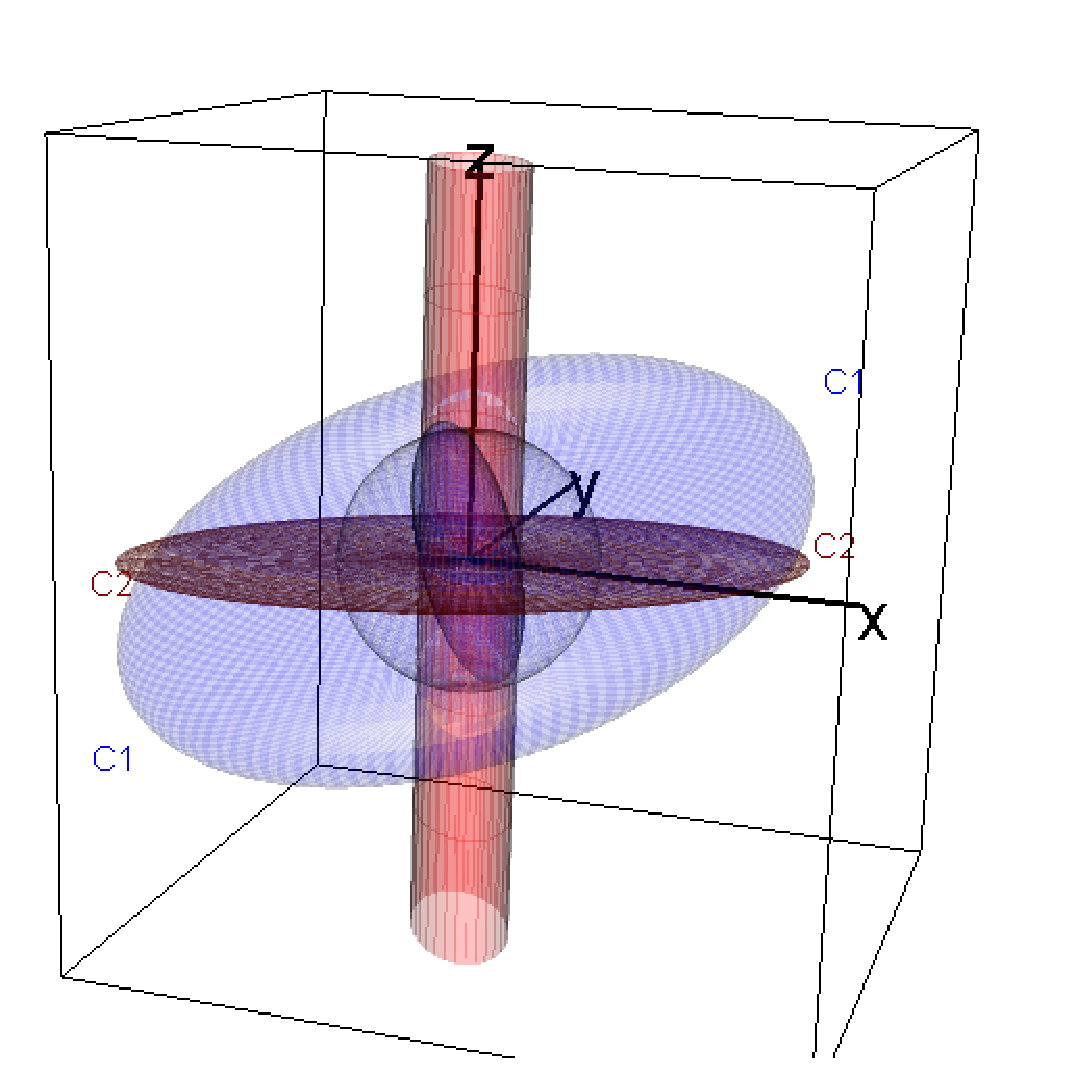
\includegraphics[width=1\linewidth]{fig/gell3d-1}
 \end{minipage}%
 \hfill
 \begin{minipage}[b]{.49\linewidth}
  \centering
  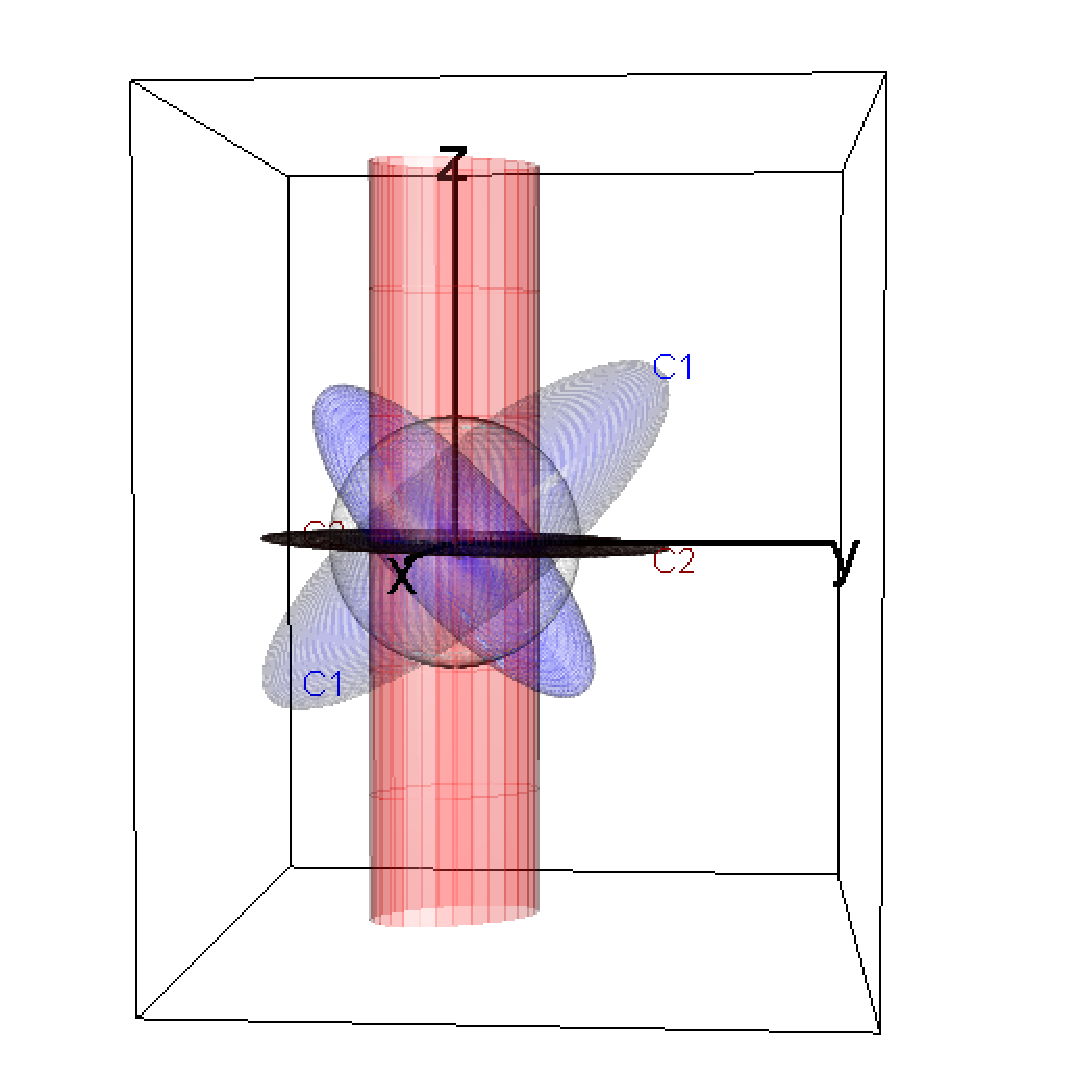
\includegraphics[width=1\linewidth]{fig/gell3d-4}
 \end{minipage}
\caption{Two views of an example of generalized ellipsoids.  $\mat{C}_1$  (blue) determines a proper, fat ellipsoid;
its inverse $\mat{C}_1^{-1}$ also generates a proper ellipsoid. $\mat{C}_2$  (red) determines an improper, flat ellipsoid,
whose inverse $\mat{C}_2^{-1}$ is an unbounded cylinder of elliptical cross section.  The scale of these images is defined
by a unit sphere (gray). The left panel shows that $\mat{C}_2$ is a projection of  $\mat{C}_1$ onto the plane where
$z=0$.
The right panel shows a view illustrating the orthogonality of each $\mat{C}$ and its dual,  $\mat{C}^{-1}$.
}
\label{fig:gell3d}
\end{figure}

The $\mat{U} (\mat{\Delta} \mathcal{S})$ representation also allow us to characterize any such
generalized ellipsoid in $\Real{p}$ by its \emph{signature},
\begin{equation}
 \mathcal{G}(\mat{C}) = \#[ \delta_i >0, \: \delta_i =0, \: \delta_i =\infty ] \quad \mbox{with} \quad \sum \mathcal{G}(\mat{C}) = p\comma
\end{equation}
a 3-vector containing the number ($\#$) of positive, zero and infinite singular values.  For example, in $\Real{3}$, any proper ellipsoid has
the signature $\mathcal{G}(\mat{C})=(3, 0, 0)$; a flat, 2D ellipsoid has $\mathcal{G}(\mat{C})=(2, 1, 0)$; a flat, 1D ellipsoid (a line)
has $\mathcal{G}(\mat{C})=(1, 2, 0)$. Unbounded examples include an infinite flat plane, with $\mathcal{G}(\mat{C})=(0, 1, 2)$,
and an infinite cylinder of elliptical cross-section, with $\mathcal{G}(\mat{C})=(2, 0, 1)$.


\figref{fig:gell3d} illustrates these ideas, using two generating matrices, $\mat{C}_1$ and $\mat{C}_2$, in this more
general representation,
\[
\mat{C}_1 = \left[
\begin{array}{ccc}
 6 & 2 & 1  \\
 2 & 3 & 2  \\
 1 & 2 & 2
\end{array}
\right]
\comma \quad\quad
\mat{C}_2 = \left[
\begin{array}{ccc}
 6 & 2 & 0  \\
 2 & 3 & 0  \\
 0 & 0 & 0
\end{array}
\right]
\]
where $\mat{C}_1$ generates a proper ellipsoid and $\mat{C}_2$ generates an improper, flat ellipsoid.
 $\mat{C}_1$ and its dual,  $\mat{C}_1^{-1}$ both have signatures $(3, 0, 0)$.
$\mat{C}_2$ has the signature $(2, 1, 0)$, while its inverse (dual) has the signature $(2, 0, 1)$.
These varieties of ellipsoids are more easily understood in the 3D movies included in the online supplements.

%\TODO{Check this section: it is complete enough? Could it be trimmed?} 
\subsection{Properties of geometric ellipsoids}\label{sec:properties}

\begin{itemize}
 \item Translation: An ellipsoid centered at $\vec{x}_0$ has the definition $\mathcal{E} := \{ \vec{x}: (\vec{x}-\vec{x}_0)\trans \mat{C} (\vec{x}-\vec{x}_0) =1
 \}$ or $\mathcal{E} := \vec{x}_0 \oplus\mat{A} \mathcal{S}$ in the notation of \secref{sec:statistical}.

 \item Orthogonality: If $\mat{C}$ is diagonal, then the origin-centered ellipsoid has its axes aligned with the coordinate axes and
has the equation
\begin{equation}\label{eq:ellisoid2}
 \vec{x}\trans \mat{C} \vec{x} = c_{11} x_1^2 + c_{22} x_2^2 + \cdots + c_{pp} x_p^2 =1 \comma
\end{equation}
where $1/\sqrt{c_{ii}} = c_{ii}^{-1/2}$ are the radii (semi-diameter lengths) along the coordinate axes.

 \item Area and volume: In two dimensions, the area of the axis-aligned ellipse is $\pi (c_{11} c_{22})^{-1/2}$.
 For $p=3$, the volume is $\frac{4}{3}\pi (c_{11} c_{22} c_{33})^{-1/2}$.
 In the general case, the hypervolume of the ellipsoid is proportional to $|\mat{C}|^{-1/2}=||\mat{A}||$
 and is given by $\pi^{p/2} \det{\mat{C}}^{-1/2} / \left[  \Gamma\left(\frac{p}{2}+1\right) \right]$
 \citep[\S 3.5]{Dempster:69}
% ($\mathcal{D}$ \S 3.5),
 where the first two factors are familiar as the normalizing constant of the multivariate normal 
 density function.

\begin{figure}[tb]
  \centering
  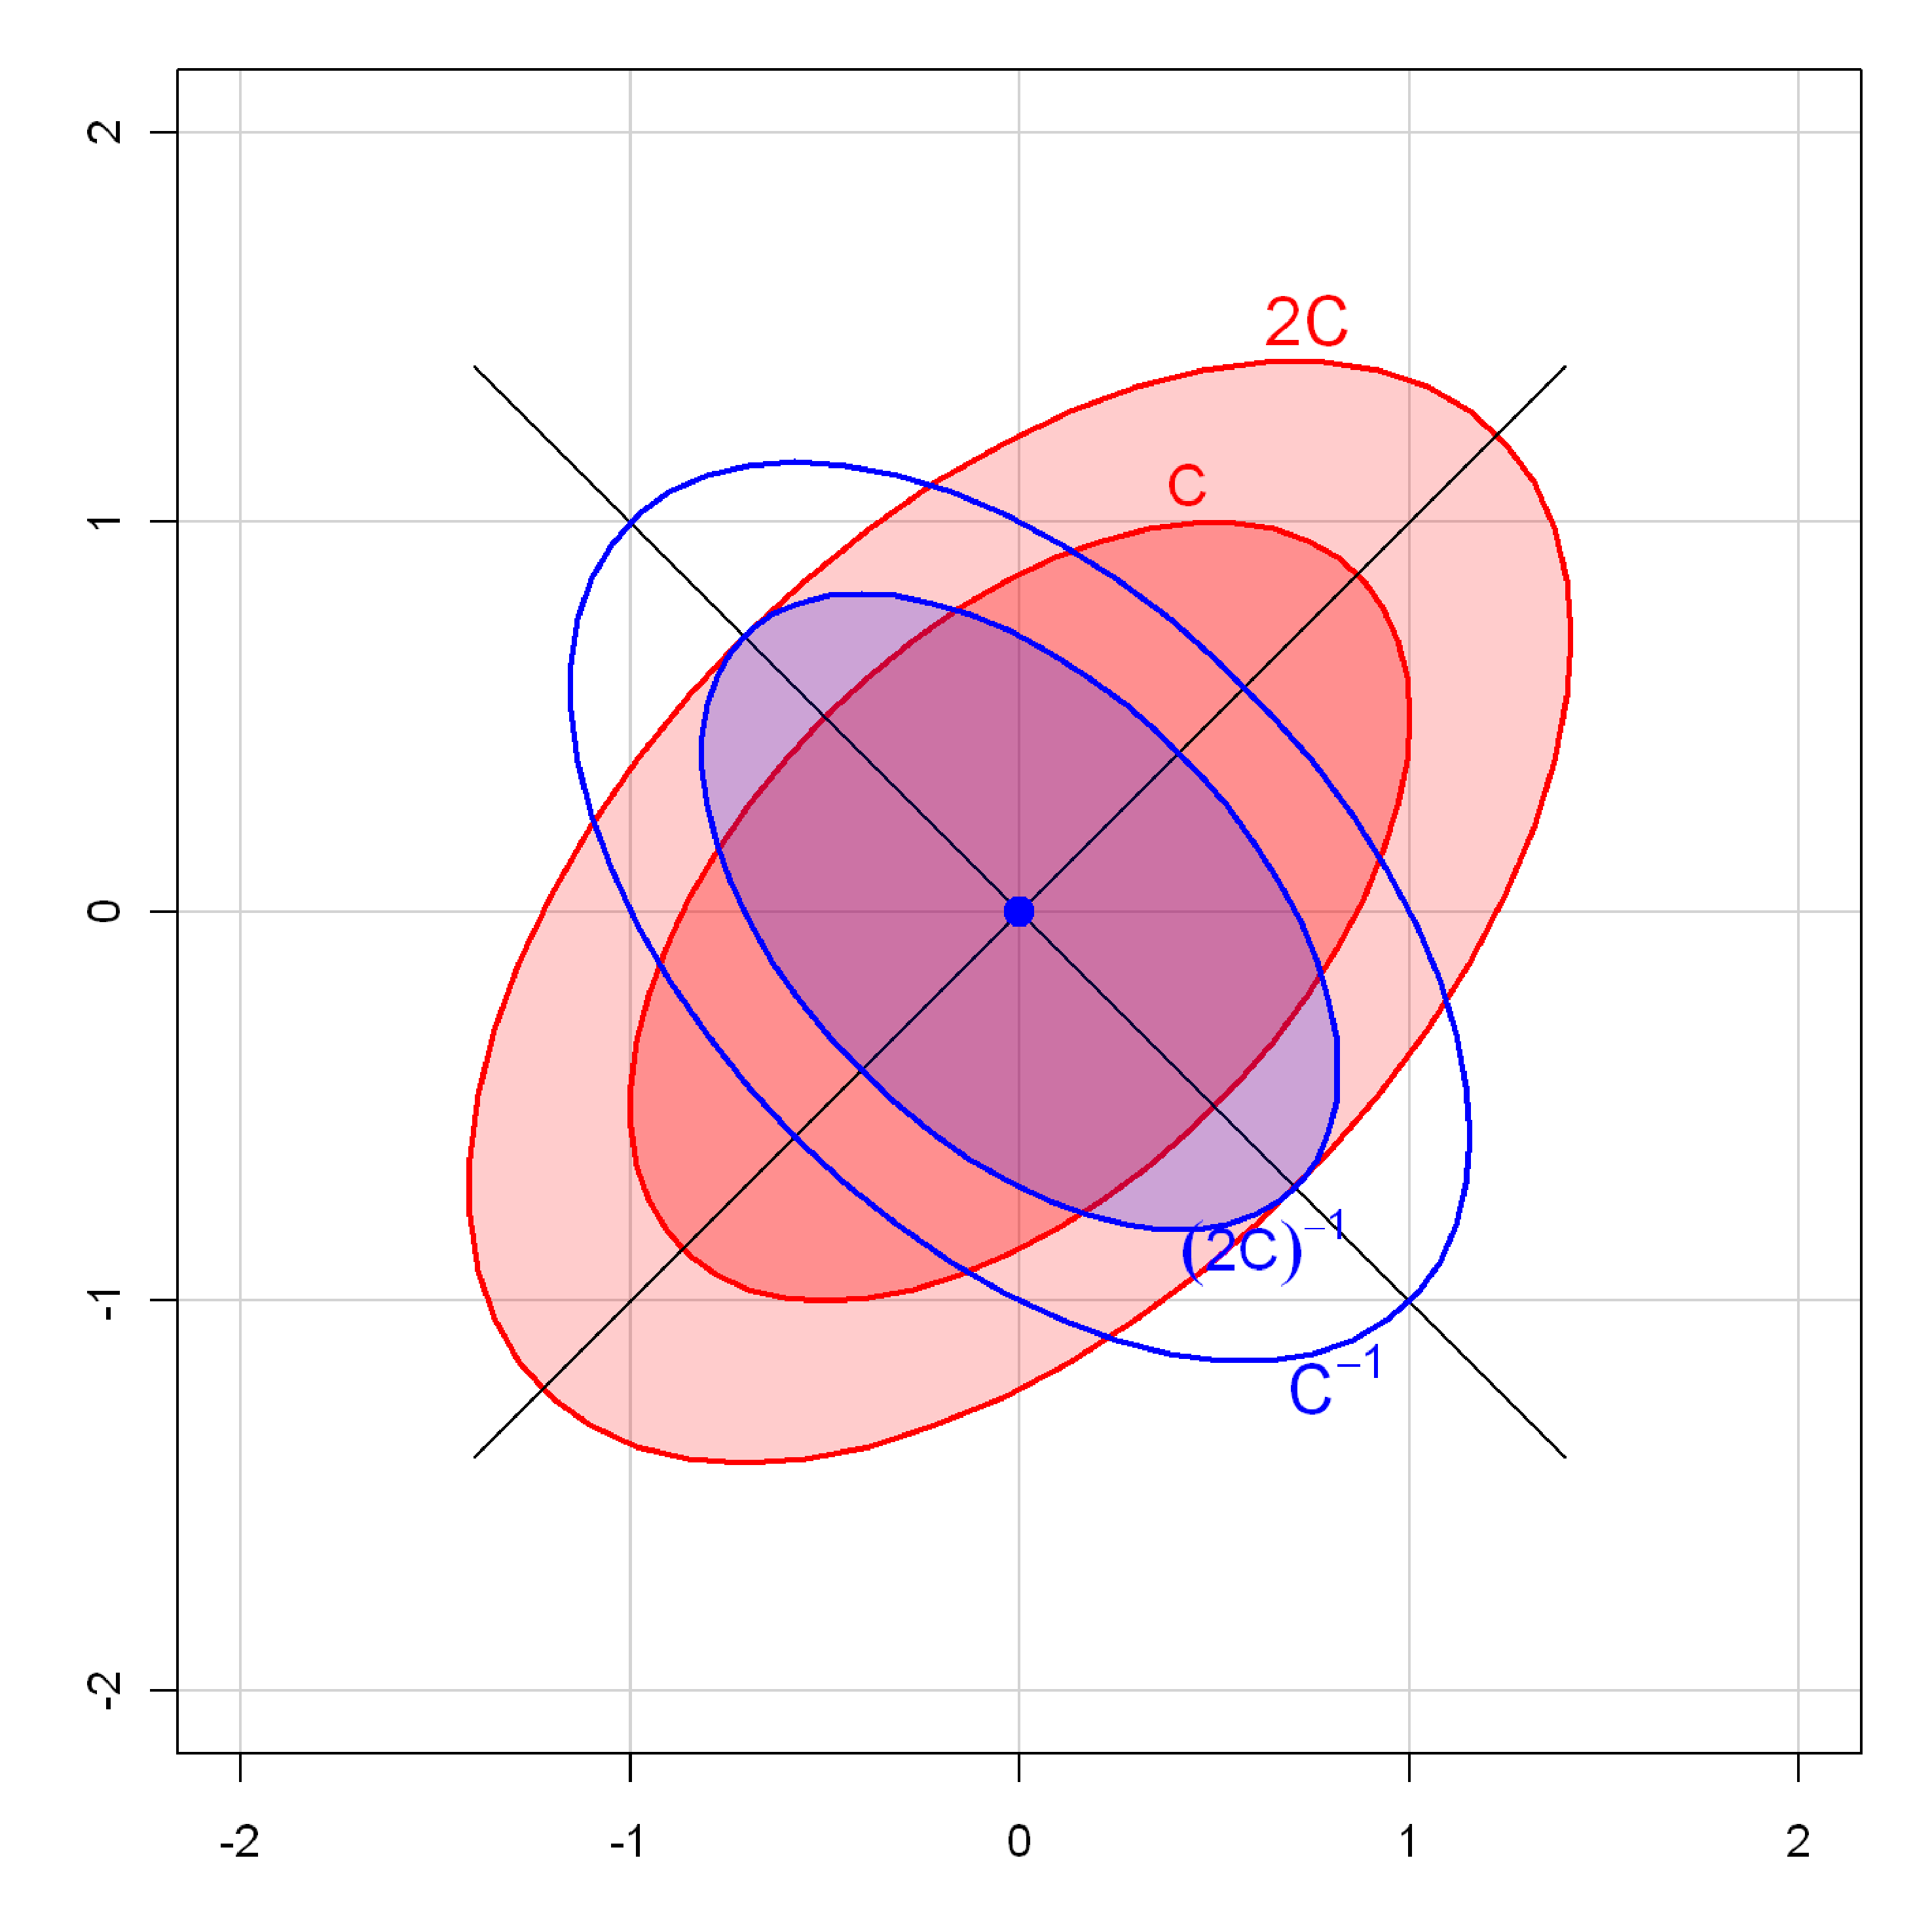
\includegraphics[width=.5\textwidth,clip]{fig/inverse}
  \caption{Some properties of geometric ellipsoids, shown in 2D. Principal axes of an ellipsoid are given by the eigenvectors of
  $\mat{C}$, with radii $1/\sqrt{\lambda_i}$.  For an ellipsoid defined by \eqref{eq:ellisoid1},
  the comparable ellipsoid for $2\mat{C}$ has radii multiplied by $1/\sqrt{2}$.
  The ellipsoid for $\mat{C}^{-1}$ has the same principal axes, but with radii $\sqrt{\lambda_i}$, making it
  small in the directions where $\mat{C}$ is large and vice-versa.
  } \label{fig:inverse}
\end{figure}

 \item Principal axes: In general, the eigenvectors, $\vec{v_i}, i=1,\dots,p$,
of $\mat{C}$ define the principal axes of the ellipsoid and
the inverse of the square roots of the ordered
eigenvalues, $\lambda_1 > \lambda_2 \dots, \lambda_p$, are the principal radii.
Eigenvectors belonging to eigenvalues that are 0 are directions in which the ellipsoid is unbounded.
With $\mathcal{E} = \mat{A} \mathcal{S}$, we consider the singular-value decomposition
$  \mat{A}= \mat{U} \mat{D} \mat{V} \trans$,
with $\mat{U}$ and  $\mat{V}$ orthogonal matrices and  $\mat{D}$  a diagonal non-negative matrix
with the same dimension as $\mat{A}$.
The column vectors of $\mat{U}$, called the left singular vectors,
correspond to the eigenvectors of $\mat{C}$ in the case of a proper ellipsoid.
The positive diagonal elements of $\mat{D}$, $d_1 > d_2 > ... > d_p>0$,
are the principal radii of the ellipsoid with $d_i = 1/\sqrt{\lambda_i}$.
In the singular case, the left singular vectors form a set of principal axes for the flattened ellipsoid.%
\footnote{Corresponding left singular vectors and eigenvectors are not necessarily equal, but sets that belong to the same eigenvalue/singular value span the same space.}

 \item Inverse: When $\mat{C}$ is positive definite, the eigenvectors of \mat{C} and $\mat{C}^{-1}$ are identical, while
the
 eigenvalues of $\mat{C}^{-1}$ are $1/\lambda_i$. It follows that the ellipsoid for
 $\mat{C}^{-1}$ has the same axes as that of $\mat{C}$, but with inversely proportional radii.
 In $\Real{2}$, the ellipsoid for $\mat{C}^{-1}$
 is, with rescaling, a \degree{90} rotation of the ellipsoid for $\mat{C}$,
 as illustrated in \figref{fig:inverse}.

 \item Generalized inverse: A definition for an inverse ellipsoid that is equivalent in the case of proper ellipsoids,
\begin{equation}\label{eq:ellipseginv}
\mathcal{E}^{-1} := \{ \vec{y} :   |\vec{x} \trans \vec{y}| \le 1 \comma \quad \forall \vec{x} \in \mathcal{E} \} \comma
\end{equation}
generalizes to all ellipsoids. The inverse of a singular ellipsoid is an improper ellipsoid and vice versa.

 \item Dimensionality: The ellipsoid is bounded if $\mat{C}$ is positive definite (all $\lambda_i > 0$).
 Each $\lambda_i = 0$ increases the dimension of the space along which the ellipsoid is unbounded by one.
For example, with $p=3$, $\lambda_3=0$ gives a
cylinder with an elliptical cross-section in 3-space, and  $\lambda_2 = \lambda_3=0$ gives an infinite slab with thickness $2 \sqrt{\lambda_1}$. With $\mathcal{E} = \mat{A} \mathcal{S}$, the dimension of the ellipsoid is equal to the number of positive singular values of $\mat{A}$.
 \item Projections: The projection of a $p$ dimensional ellipsoid into any subspace
is $\mat{P} \mathcal{E}$, where
$\mat{P}$ is an idempotent $p \times p$ (projection) matrix, i.e., $\mat{P} \mat{P}= \mat{P}^2 = \mat{P}$.
For example, in $\Real{2}$ and $\Real{3}$,
% $\Re^3$,
the matrices
\[
\mat{P}_2 =
\left[
\begin{array}{cc}
 1 & 1  \\
 0 & 0  \\
\end{array}
\right]
\comma \quad\quad
\mat{P}_3 =
\left[
\begin{array}{ccc}
 1 & 0 & 0 \\
 0 & 1 & 0 \\
 0 & 0 & 0 \\
\end{array}
\right]
\]
project, respectively, an ellipse onto the line $x_1 = x_2$, and an ellipsoid into the ($x_1, x_2$) plane.  If $\mat{P}$ is symmetric, then $\mat{P}$ is the matrix of an orthogonal projection, and it is easy to visualize  $\mat{P} \mathcal{E}$ as the shadow of  $\mathcal{E}$ cast perpendicularly onto  $\mathrm{span}(\mat{P})$. Generally,  $\mat{P} \mathcal{E}$ is the shadow of $\mathcal{E}$  onto  $\mathrm{span}(\mat{P})$ along the null space of $\mat{P}$.

 \item Linear transformations: A linear transformation of an ellipsoid is an ellipsoid, and the pre-image of an ellipsoid under a linear transformation is an ellipsoid.  
A non-singular linear transformation maps a proper ellipsoid into a proper ellipsoid in the form shown in \secref{sec:statistical}, \eqref{eq:Limage}. 

 \item Slopes and tangents: The slopes of the ellipsoidal surface in the directions of the coordinate
 axes are given by $\partial / \partial \vec{x} \: (\vec{x}\trans \mat{C} \vec{x}) = 2 \mat{C} \vec{x}$.
 From this, it follows that the tangent hyperplane to the unit ellipsoidal surface at the point
 $\vec{x}_\alpha$, where $\vec{x}_\alpha\trans \: \partial / \partial \vec{x} (\vec{x}\trans \mat{C} \vec{x}) = 0$,
 has the equation $\vec{x}_\alpha \trans \mat{C} \vec{x} = 1$.
\end{itemize}


\subsection{Conjugate axes and inner-product spaces}\label{sec:conjugate}

For any non-singular $\mat{A}$ in \eqref{eq:ellAS} that generates an ellipsoid,  %% added non-singular / GM
the columns of
$\mat{A}=\left[
   \vec{a}_{1}, \vec{a}_{2}, \cdots, \vec{a}_{p}  \\
\right]
$
form a set of ``conjugate axes'' of the ellipse. (Two diameters are conjugate \emph{iff}
the tangent line at the endpoint of one diameter is parallel to the other diameter.)
Each vector
$\vec{a}_{i}$
lies on the ellipse, and the tangent hyperplane at that point is parallel to the span of all the other column vectors of
$\vec{A}$.
\begin{figure}[htb]
 \begin{minipage}[b]{.49\linewidth}
  \centering
  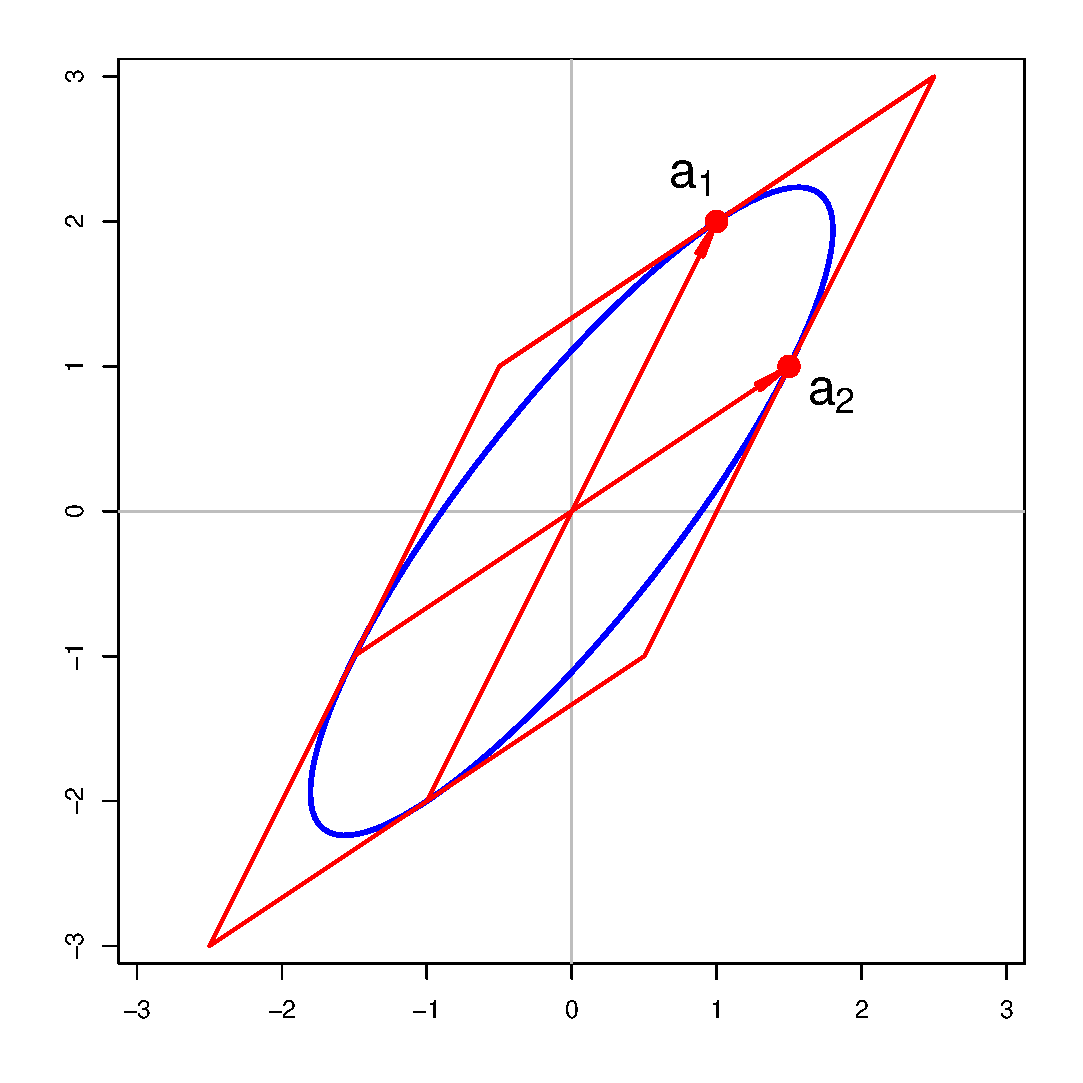
\includegraphics[width=1\linewidth]{fig/conjugate1}
 \end{minipage}%
 \hfill
 \begin{minipage}[b]{.49\linewidth}
  \centering
  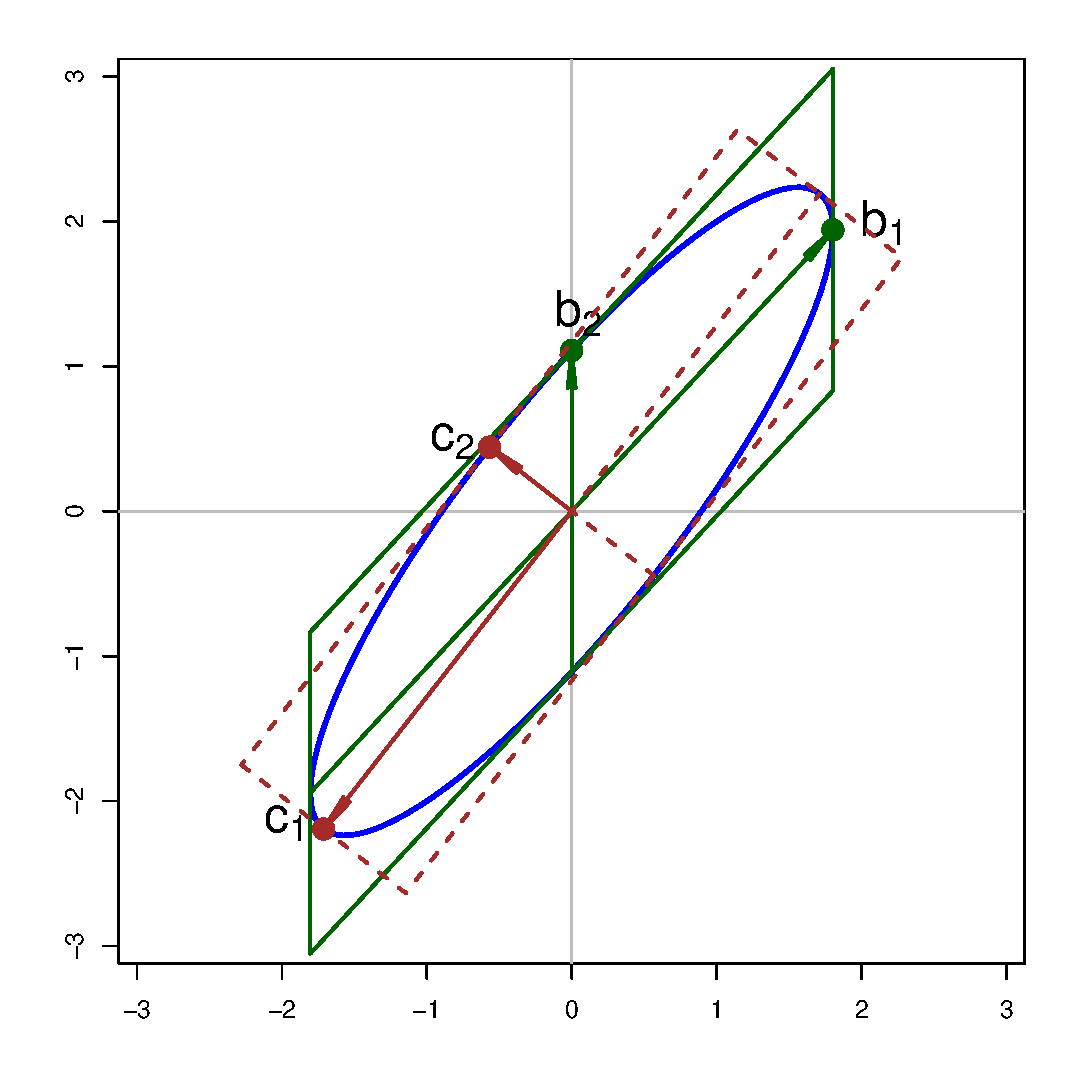
\includegraphics[width=1\linewidth]{fig/conjugate2}
 \end{minipage}
\caption{Conjugate axes of an ellipsoid with various factorizations of $\mat{W}$ and corresponding
basis vectors.
The conjugate vectors lie on the ellipsoid, and their tangents can be extended to form a parallelogram framing it.
Left: for an arbitrary factorization, given in \eqref{eq:fac1}.
Right: for the Choleski factorization (solid, green, $b_1, b_2$) and the principal component factorization (dashed, brown, $c_1, c_2$).
}
\label{fig:conjugate}
\end{figure}
For
$p=2$
this result is illustrated in \figref{fig:conjugate} (left)
in which

\begin{equation}\label{eq:fac1}
\mat{A}=\left[ \begin{matrix}
   \vec{a}_{1} & \mat{a}_{2}  \\
\end{matrix} \right]=\left[
\begin{matrix}
   1 & 1.5  \\
   2 & 1  \\
\end{matrix} \right]
\mbox{   }\Rightarrow\mbox{   }
\mat{W}=\mat{A A\trans}=
\left[ \begin{matrix}
   3.25 & 3.5  \\
   3.5 & 5  \\
\end{matrix} \right]
\period
\end{equation}

Consider the inner-product space with inner product matrix 	
$\mat{W}^{-1}=\left[ \begin{matrix}	
1.25 & -0.875 \\	
-0.875 & 0.8125 \\	
\end{matrix} \right]
$ and inner product	
\begin{equation*}
\left\langle \vec{x},\vec{y} \right\rangle =\vec{{x}'W}^{-1}\vec{y} \period
\end{equation*} 	
Because	
$\mat{A}\trans \mat{W}^{-1}\mat{A}
=\mat{A}\trans\left( \mat{A}\mat{A}\trans \right)^{-1}\mat{A}
=\mat{A}\trans(\mat{A}\trans)^{-1}\mat{A}^{-1}\mat{A}
=\mat{I}
$,
we see that
$\vec{a}_{1}$
and	
$\vec{a}_{2}$	
are orthogonal unit vectors (in fact, an orthonormal basis) in this inner product:	

\begin{eqnarray*}
\left\langle \vec{a}_{i},\vec{a}_{i} \right\rangle & = & \vec{{a}\trans}_{i}\mat{W}^{-1}\vec{a}_{i}=1	 \\
%	
\left\langle \vec{a}_{1},\vec{a}_{2} \right\rangle & = &\vec{{a}'}_{1}\mat{W}^{-1}\vec{a}_{2}=0 \period
\end{eqnarray*}


Now, if $\mat{W}=\mat{B{B}\trans}$ is any other factorization of
$\mat{W}$,
then the columns of
$\mat{B}$
have the same properties as the columns of
$\mat{A}$.
Particular factorizations yield interesting and statistically useful sets of conjugate axes.
The illustration in \figref{fig:conjugate} (right) shows two such cases with special properties:
In the Choleski factorization (shown solid in green), where
$\mat{B}$ is lower triangular, the last conjugate axis, $\vec{b}_2$, is aligned with the coordinate
axis $\vec{x}_2$.  Each previous axis ($\vec{b}_1$, here) is the orthogonal complement to
all later axes in the  inner-product space of
$\mat{W}^{-1}$.  
The Choleski factorization is unique in this respect, subject to a
permutation of the rows and columns of \mat{W}. 
The subspace $\{ c_1 \vec{b}_1 + ... + c_{p-1} \vec{b}_{p-1}  , c_i \in \mathbb{R}\}$, is the plane of the regression of the last variable on the others, a fact that generalizes naturally to ellipsoids that are not necessarily centerered at the origin.  %% added fact /GM  

In the principal-component (PC) factorization (shown dashed in brown) $\mat{W}=\mat{C} \mat{C}\trans$, where
$\mat{C}=\mat{\Gamma \Lambda }^{1/2}$
and hence
$\mat{W}=\mat{\Gamma \Lambda {\Gamma }'}$
is the spectral decomposition of
$\mat{W}$. Here, the ellipse axes are orthogonal in the space of the ellipse
(so the bounding tangent parallelogram is a rectangle) \emph{as well as} in the inner-product space of
$\mat{W}^{-1}$. The PC factorization is unique in this respect (up to reflections of the axis vectors).

As illustrated in \figref{fig:conjugate}, each pair of conjugate axes has a corresponding bounding tangent
parallelogram. It can be shown that all such parallelograms have the same area
and equal sums of squares of the lengths of their diameters.

\subsection{Ellipsoids in a generalized metric space}

%\todo{Georges?}
%\TODO{Smooth out and simplify this description. Add to the plot: unit vectors in data space, and their transformations in canonical space.
%Here it would be useful to describe the geometric relations that pertain to \mat{H}
%(positive semi-definite)
%in the metric of \mat{E} (positive definite).
%I see two sub-figures:
%(a) ellipses for \mat{H} and \mat{E}, showing the conjugate axes and
%bounding parallelogram for \mat{E}, perhaps using the principal component factorization.
%(b) the transformation of (a) using $\mat{H}\mat{E}^{-1}$ or
%$\mat{E}^{-1/2} \, \mat{H} \, \mat{E}^{-1/2}$.
%}

In the discussion above, we considered the positive semi-definite matrix \mat{W} and
corresponding ellipsoid to be
referred to a Euclidean space, perhaps with different basis vectors.
We showed that various measures of the ``size'' of the ellipsoid could be defined
in terms of functions of the eigenvalues $\lambda_i$ of \mat{W}.

We now consider the generalized
case of an analogous $p \times p$ positive semi-definite symmetric matrix \mat{H}, but where measures of
length, distance, and angles are referred to a metric defined by a positive-definite symmetric
matrix \mat{E}. As is well known, the generalized eigenvalue problem is to find the scalars
$\lambda_i$ and vectors $\vec{v}_i, i=1, 2, \dots p$,
such that $\mat{H} \vec{v} = \lambda \mat{E} \vec{v}$, that is, the roots of
$\det{\mat{H} - \lambda \mat{E}}=0$.

%\TODO{More explanation here ...}
\begin{figure}[htb]
% two figs side-by-side
  \begin{minipage}[c]{.495\textwidth}
   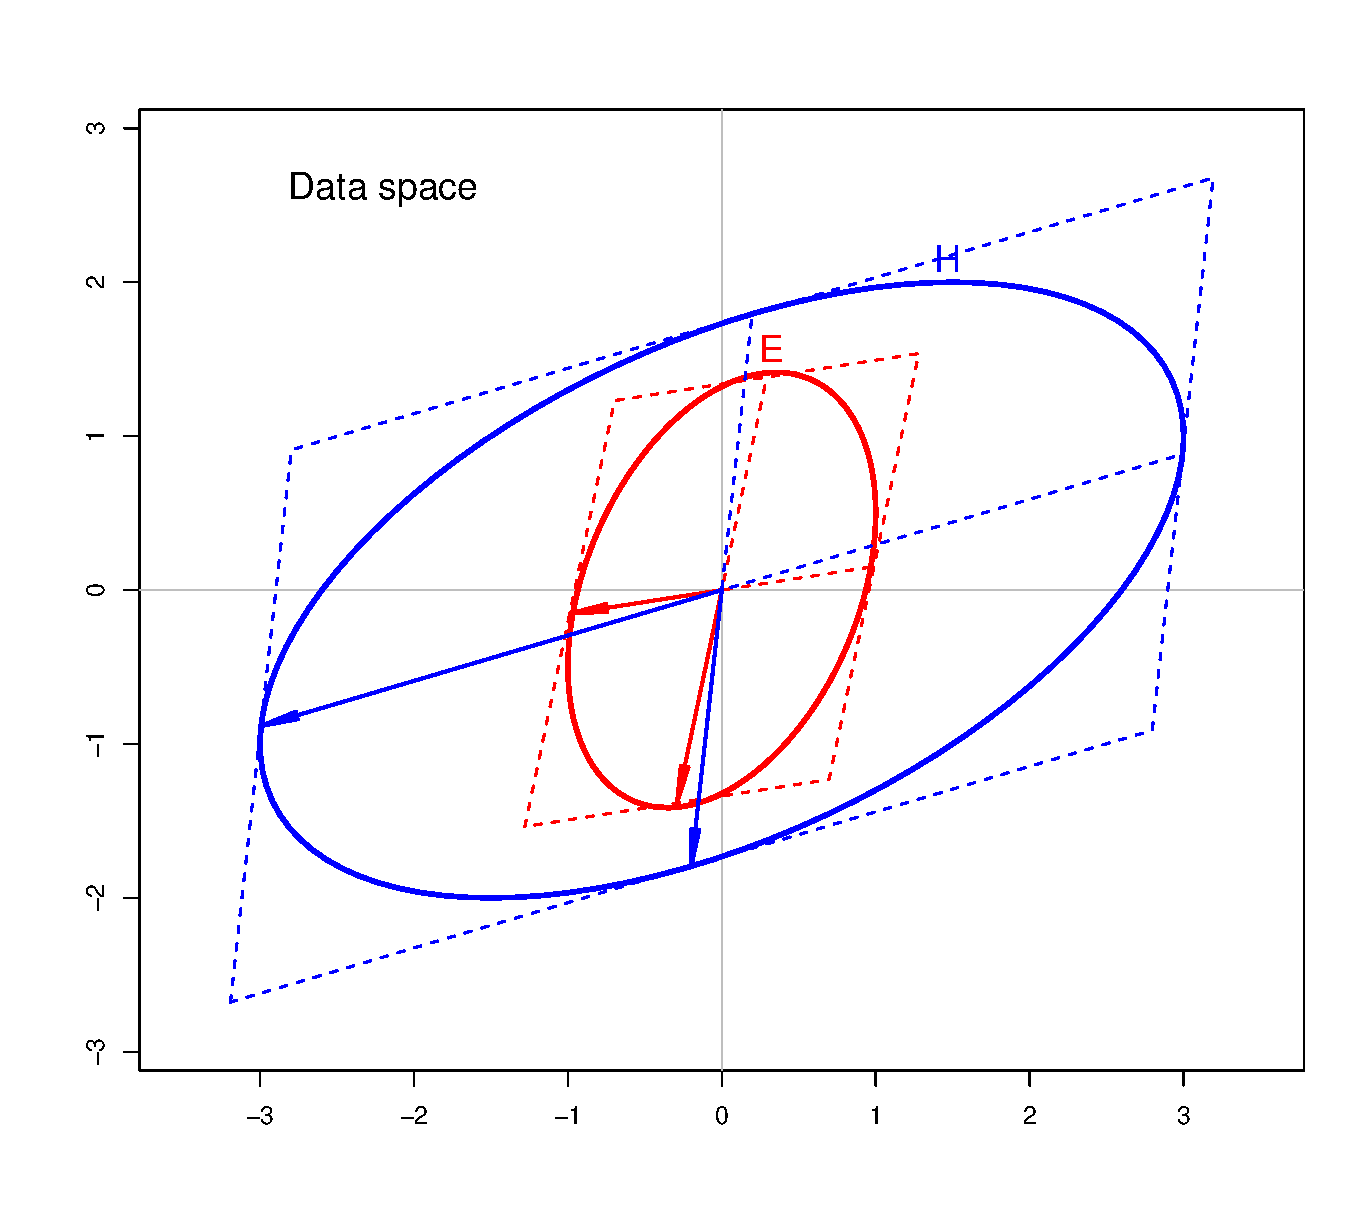
\includegraphics[width=1\linewidth,clip]{fig/ellipse-geneig1}
   \end{minipage}%
  \hfill
  \begin{minipage}[c]{.495\textwidth}
   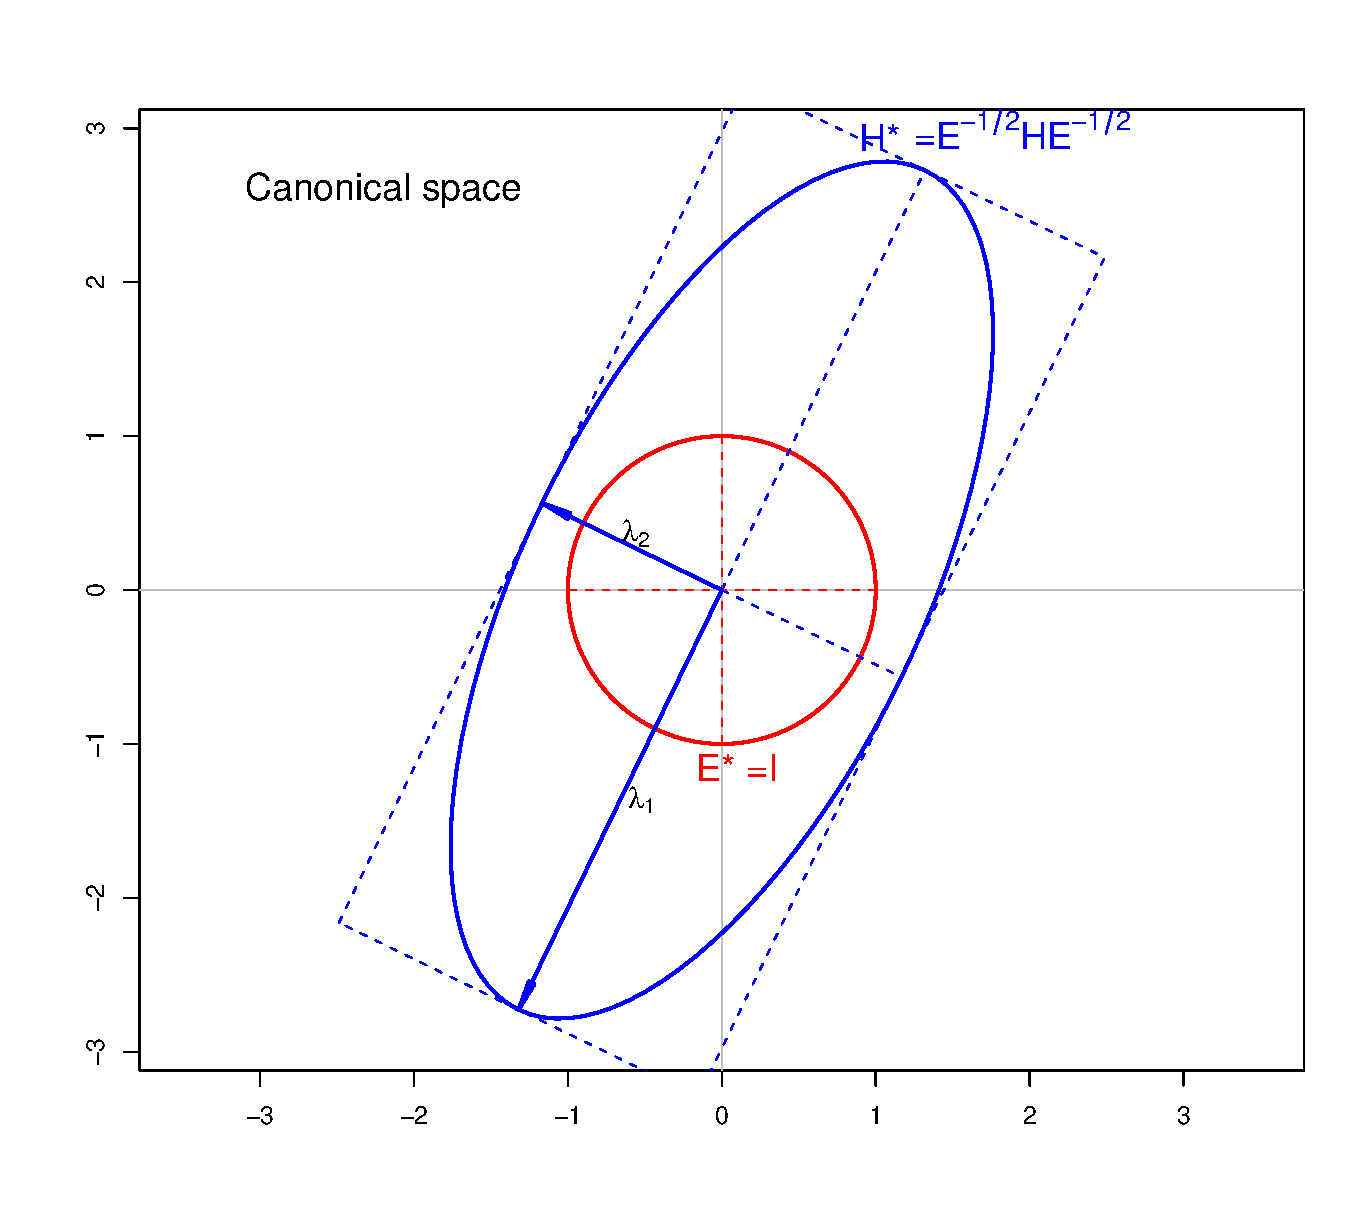
\includegraphics[width=1\linewidth,clip]{fig/ellipse-geneig2}
  \end{minipage}
  \caption{Left: Ellipses for \mat{H} and \mat{E} in Euclidean ``data space,''
   Right: Ellipses for $\mat{H}^\star$ and $\mat{E}^\star$ in the transformed ``canonical space,''
   with the eigenvectors of \mat{H} relative to \mat{E} shown as blue arrows, whose radii
   are the corresponding eigenvalues, $\lambda_1, \lambda_2$. }%
  \label{fig:ellipse-geneig}
\end{figure}
For such \mat{H} and \mat{E}, we can always find a factor \mat{A} of \mat{E}, so that
$\mat{E} = \mat{A} \mat{A}\trans$, whose colums will be conjugate directions for \mat{E}
and whose rows will also be conjugate directions for \mat{H}, in that $\mat{H} = \mat{A}\trans \mat{D} \mat{A}$,
where $\mat{D}$ is diagonal.  Geometrically, this means that there exists a unique pair of
bounding parallelograms for the \mat{H} and \mat{E} ellipsoids whose
corresponding sides are parallel. A linear transformation of \mat{E} and \mat{H}
that transforms the parallelogram
for \mat{E} to a square (or cuboid), and hence \mat{E} to a sphere (or spheroid), generates an
equivalent view in what we describe below as canonical space.


In statistical applications (e.g., MANOVA, canonical correlation), the generalized
eigenvalue problem is transformed to an ordinary eigenvalue problem by considering
the following equivalent forms with the same $\lambda_i$, $\vec{v}_i$,
\begin{eqnarray*}
(\mat{H} - \lambda \mat{E}) \vec{v} & = & \vec{0} \\
\Rightarrow (\mat{H} \, \inv{\mat{E}} - \lambda \mat{I}) \vec{v} & = & \vec{0} \\
\Rightarrow (\invhalf{\mat{E}} \, \mat{H} \, \invhalf{\mat{E}} - \lambda \mat{I}) \vec{v} & = & \vec{0} \comma
\end{eqnarray*}
where the last form gives a symmetric matrix, $\mat{H}^\star = \invhalf{E} \, \mat{H} \, \invhalf{E}$.
Using the square root of \mat{E} defined by the
principal-component factorization $\half{E} = \mat{\Gamma} \half{\mat{\Lambda}}$ produces
the ellipsoid of $\mat{H}^\star$
orthogonal axes corresponding to the $\vec{v}_i$, whose squared radii are the corresponding %% squared / GM
eigenvalues $\lambda_i$.  This can be seen geometrically as a rotation of ``data space''
to an orientation defined by the principal axes of \mat{E}, followed by a re-scaling, so
that the \mat{E} ellipsoid becomes the unit spheroid.  In this transformed space
(``canonical space''), functions of the
the squared radii $\lambda_i$ of the axes of $\mat{H}^\star$ give direct measures of %% squared / GM
the ``size'' of \mat{H} relative to \mat{E}. The orientation of the eigenvectors
$\vec{v}_i$ can be related to the (orthogonal) linear combinations of the
data variables that are successively largest in the metric of \mat{E}.


To illustrate, \figref{fig:ellipse-geneig} (left) shows
the ellipses generated by
\begin{equation*}
 \mat{H} = \left[ \begin{array}{cc}
                   9 & 3 \\
                   3 & 4
                  \end{array}\right]
 \quad \mbox{ and } \quad
 \mat{E} = \left[ \begin{array}{cc}
                   1 & 0.5 \\
                   0.5 & 2
                  \end{array}\right]
\end{equation*}
together with their conjugate axes. For \mat{E}, the conjugate axes are defined by the columns of the right factor,
$\mat{A}\trans$,
in $\mat{E} = \mat{A} \mat{A}\trans$; for \mat{H}, the conjugate axes are defined by the columns of $\mat{A}$.
The transformation to $\mat{H}^\star = \invhalf{E} \, \mat{H} \, \invhalf{E}$ is shown in the right panel
of \figref{fig:ellipse-geneig}. In this ``canonical space,'' angles and lengths have the orginary interpretation
of Euclidean space, so the size of $\mat{H}^\star$ can be interpreted directly in terms of functions of
the radii $\sqrt{\lambda_1}$ and $\sqrt{\lambda_2}$.



\section{SAS and R code for figures}\label{sec:SASandR}

We provide the source code used to generate all of the figures with this supplement in the file
\newline
\file{ellipses-suppfiles.zip}.
It should
be noted that these illustrations were developed over a considerable period of time, using a collection
of general SAS macro programs and R packages by the authors and others (listed below). It often happened
that these software tools were not sufficiently general or capable for our purposes.  In many cases the
SAS macros and R packages were extended (or a new package was written, e.g., 
the \pkg{genridge} package \citep{genridge,Friendly:genridge:2012} for the material on ridge trace plots in
\secref{sec:ridge2})
to make these analyses and figures easier to do in the future. Once we enhanced the SAS macros
or R packages, however, we did not often go back and re-do the figures using the revised tools.  

\subsection{Macros and R packages}
The SAS programs use a collection of SAS macros, available from the website \url{http://datavis.ca/sasmac/}.
See  \url{http://datavis.ca/books/sssg/usage.html} for installation and usage notes.

The following R packages beyond those standardly installed with R itself are available from any
CRAN mirror site, e.g., \url{http://cran.us.r-project.org}:
\pkg{candisc}, \pkg{car}, \pkg{ellipse}, \pkg{heplots}, \pkg{mvmeta}, \pkg{sfsmisc}.
Three other packages, still under development by the authors are available from the R-Forge server,
\url{http://r-forge.r-project.org}: \pkg{p3d} \citep{p3d} and \pkg{spida} \citep{spida};
\pkg{gellipsoid} implements generalized ellipsoids as described in \appref{sec:Appendix}.

\subsection{Visual directory for figures}
SAS and R source files are contained in the directories \file{SAS/} and \file{R/} respectively.
The table below shows thumbnails of the figures together with the name of the 
corresponding SAS or R source file.
\newcommand{\Figure}[3]{%
  \begin{tabular}[b]{c}
    Fig. #1 \\\textbf{#3} \\ \includegraphics[width=.2\textwidth,clip]{#2} 
\end{tabular} 
}

\begin{longtable}{cccc}
\hline
\multicolumn{4}{c}{\textbf{\large Paper}} \\ \hline
\Figure{ 2}{fig/galton-reg3}{SAS/galton-reg3.sas}       &
\Figure{ 3}{fig/scatirisd1}{SAS/scatirisd.sas}          &
\Figure{ 4}{fig/ellipses-demo}{R/ellipses-demo.R}       &
\Figure{ 5}{fig/vis-reg-prestige1}{R/vis-reg-prestige.R} \\ \hline
\Figure{ 6}{fig/contiris3}{SAS/contiris.sas}            &
\Figure{ 7}{fig/between-within1}{R/between-within.R}    &
\Figure{ 8}{fig/between-HE1}{R/between-within.R}        &
\Figure{ 9}{fig/levdemo21}{SAS/levdemo2.sas}             \\  \hline       
\Figure{11}{fig/vis-reg-coffee11}{R/vis-reg-coffee1.R}  &
\Figure{12}{fig/vis-reg-coffee12a}{R/vis-reg-coffee1.R} &
\Figure{13}{fig/vis-reg-coffee13}{R/vis-reg-coffee1.R}  &
\Figure{14}{fig/coffee-stress1}{R/coffee-stress.R}        \\ \hline
\Figure{15}{fig/coffee-measerr}{R/coffee-measerr.R}     &
\Figure{16}{fig/coffee-avplot1}{R/coffee-avPlots.R}     &
\Figure{17}{fig/coffee-av3D-1}{R/coffee-av3D.R}         &
\Figure{18}{fig/coffee-avplot3}{R/coffee-avPlots.R}       \\ \hline
\Figure{19}{fig/mtests}{R/mtests.R}                     &
\Figure{20}{fig/heplot3a}{SAS/heplot3a.sas}             &
\Figure{21}{fig/HE-contrasts-iris}{R/HE-contrasts-iris.R} &
\Figure{22}{fig/HE-can-iris}{R/HE-can-iris.R}             \\ \hline
\Figure{23}{fig/kiss-demo}{R/kiss-demo.R}               &
\Figure{24}{fig/kiss-demo2a}{R/kiss-demo2.R}            &
\Figure{25}{fig/ridge-demo}{R/ridge-demo.R}             &
\Figure{26}{fig/ridge2}{R/ridge2.R}                        \\ \hline   
\Figure{27}{fig/hsbmix41}{SAS/hsbmix4.sas}              &
\Figure{28}{fig/hsbmix43}{SAS/hsbmix4.sas}              &
\Figure{29}{fig/mvmeta2a}{R/mvmeta2.R}                  &  \\ \hline
% 
\hline
\multicolumn{4}{c}{\textbf{\large Appendix}} \\ \hline
\Figure{A.1}{fig/gell3d-1}{R/gell3d.R}                  &
\Figure{A.2}{fig/inverse}{R/inverse.R}                  &
\Figure{A.3}{fig/conjugate1}{R/conjugate.R}             &
\Figure{A.4}{fig/ellipse-geneig1}{R/ellipse-geneig.R}      \\
\hline
%\end{tabular}
\end{longtable}

\section{Movies}\label{sec:movies}
Several 3D figures in the paper or this supplementary Apppendix are rendered as static images from different views
in the print version.  These figures include \figref{fig:coffee-av3D} and \figref{fig:gell3d}, reproduced below.

\begin{figure}[htb]
 \begin{minipage}[b]{.49\linewidth}
  \centering
  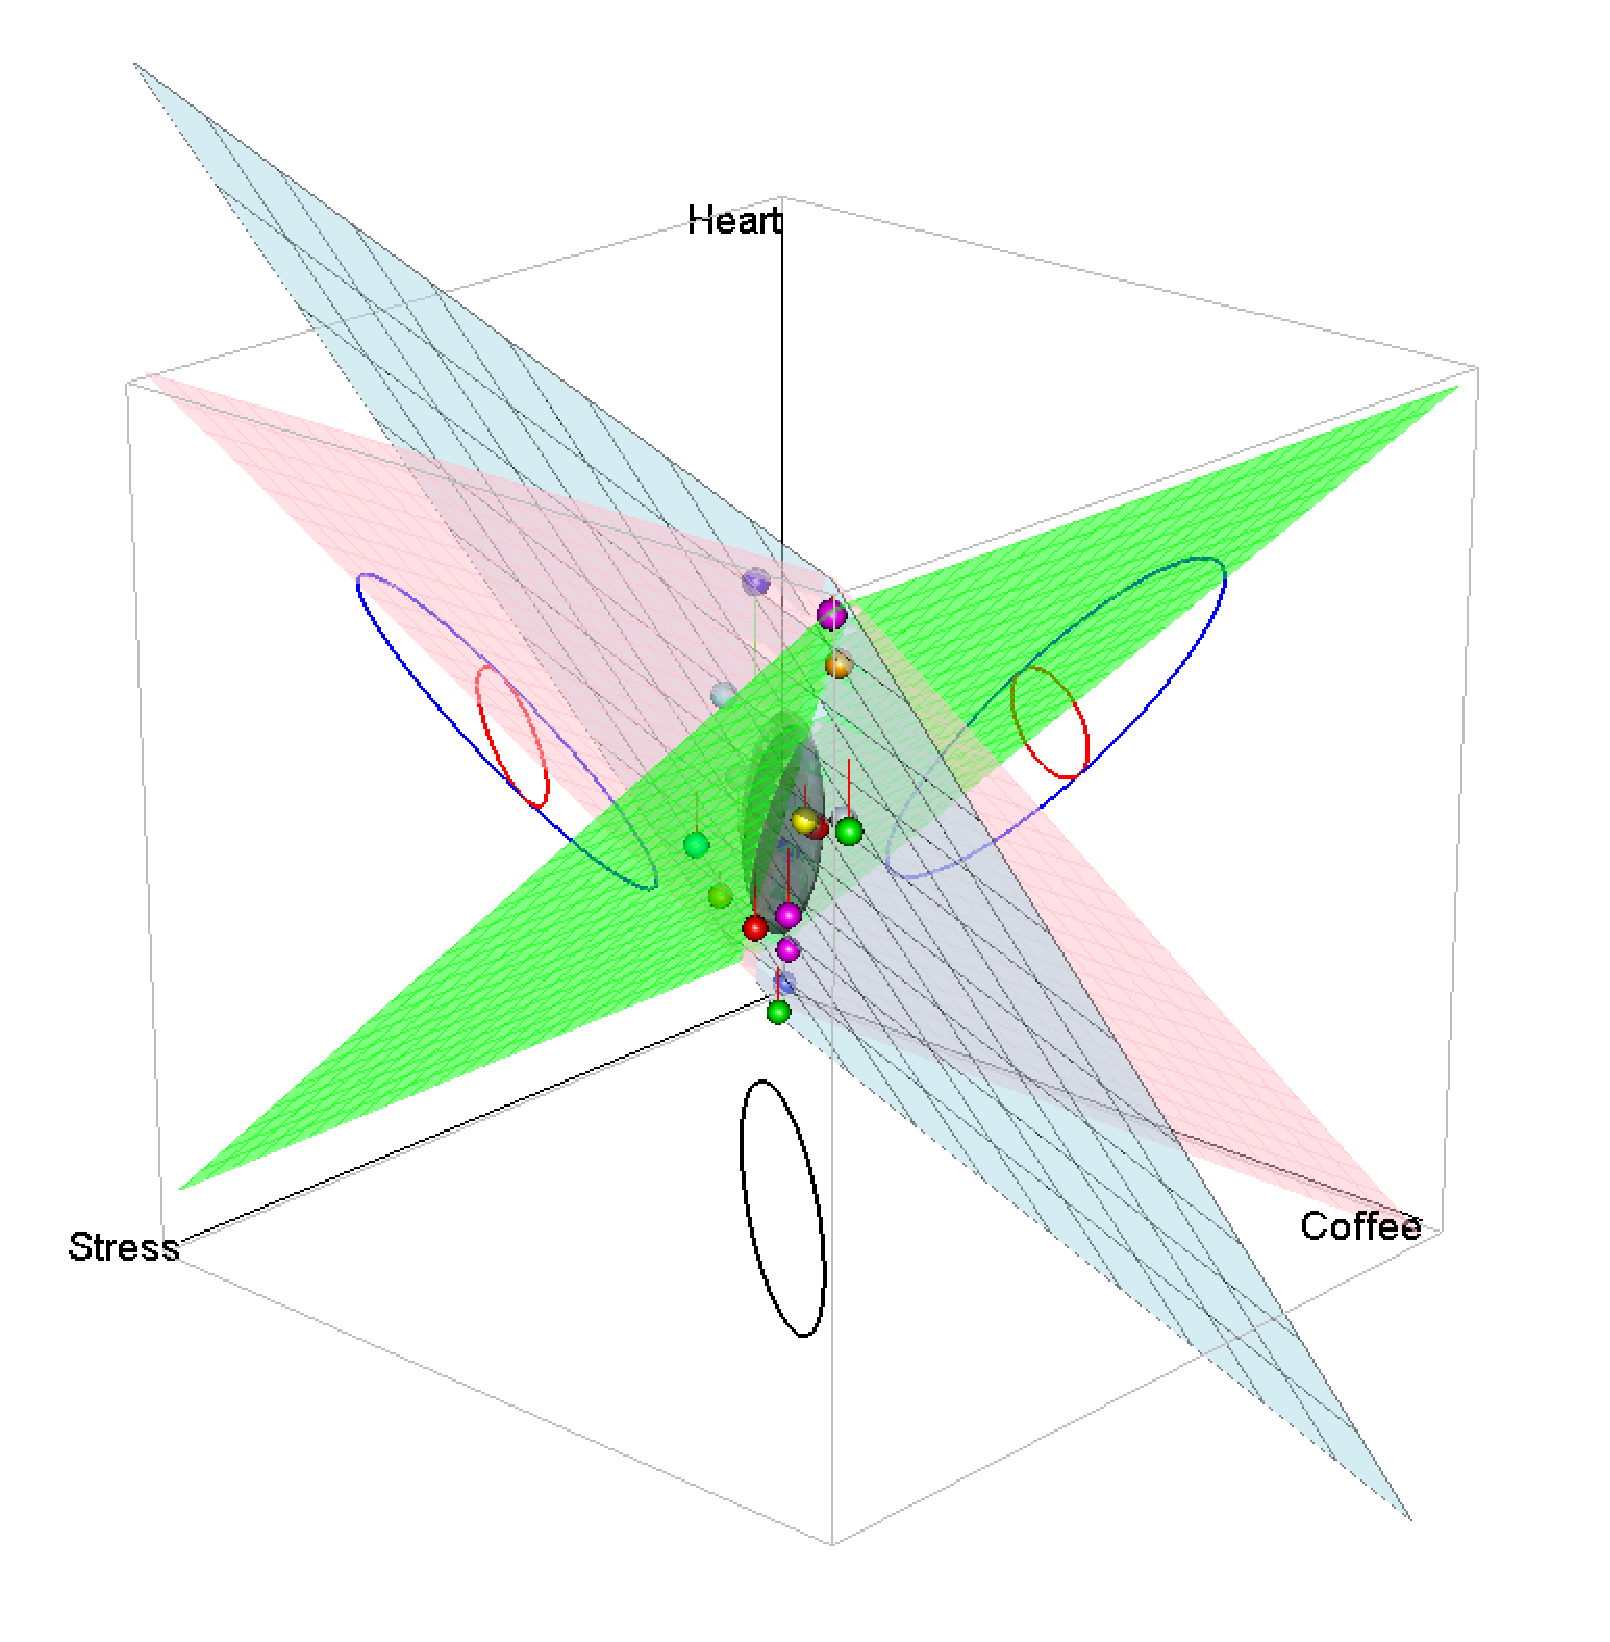
\includegraphics[width=1\linewidth]{fig/coffee-av3D-1}
%  \caption{}%
%  \label{fig:}
 \end{minipage}%
 \hfill
 \begin{minipage}[b]{.49\linewidth}
  \centering
  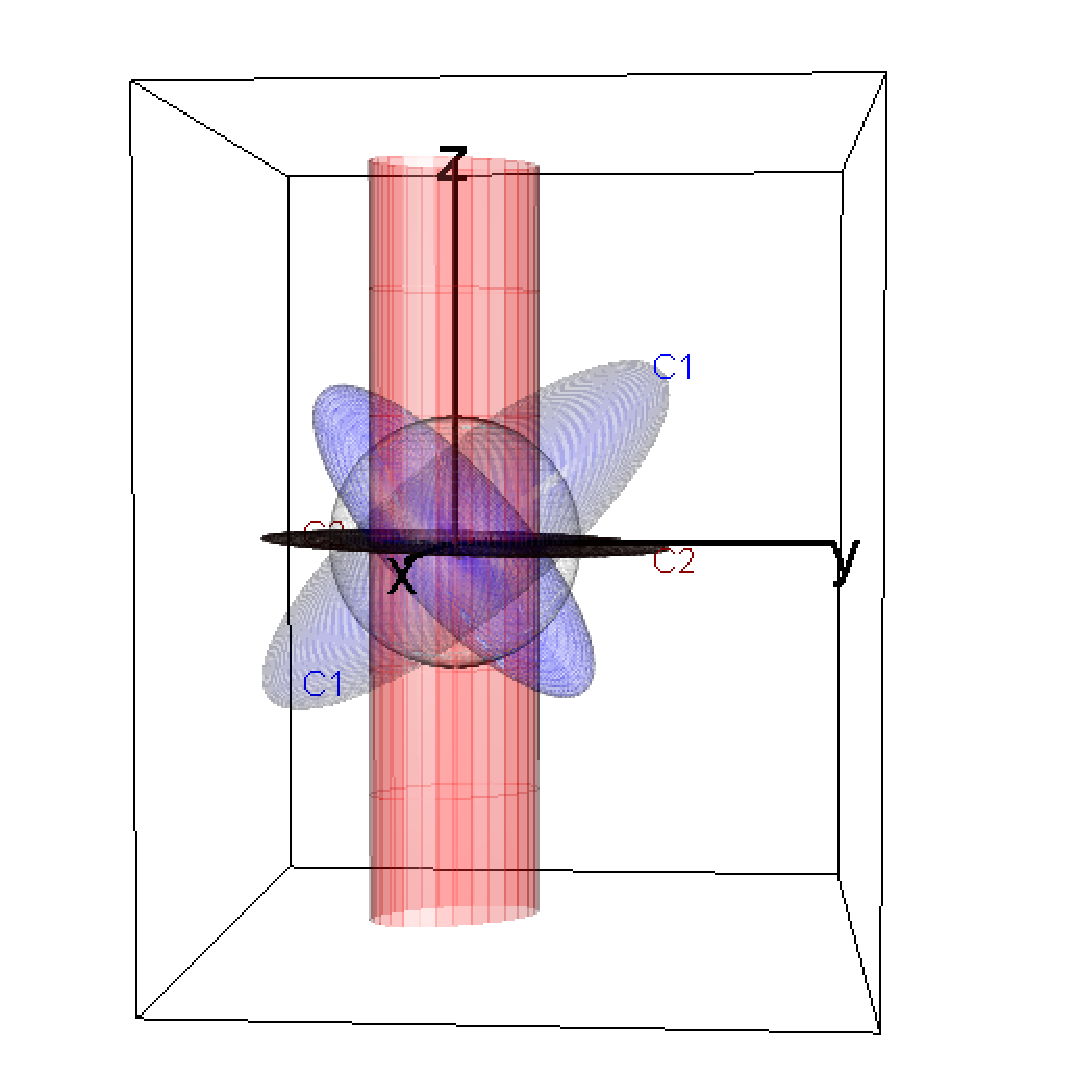
\includegraphics[width=1\linewidth]{fig/gell3d-4}
 \end{minipage}
  \caption{Left: 3D view of the relationship between Heart, Coffee and Stress, from \figref{fig:coffee-av3D} in the paper; source: \file{R/coffee-av3D.R}.
  Right: 3D view of an example of generalized ellipsoids, from \figref{fig:gell3d}: source: \file{R/gell3d.R}.  
  }
  \label{fig:supp3D}
\end{figure}

These were generated using the \pkg{rgl} package in R \citep{rgl}, 
which allows such 3D views to be rotated, zoomed
and otherwise manipulated in 3D space manually, and also supports making animated movies. The movies we created
are contained in the \file{movies/} directory.

% \appendix
% \numberwithin{equation}{section}
% \numberwithin{figure}{section}
% \section{Geometrical and statistical ellipsoids}\label{sec:Appendix}
% This appendix outlines useful results and properties concerning the representation of geometric and statistical ellipsoids.
% A number of these can be traced to or have more general descriptions within the abstract formulation of \citet{Dempster:69},
% (henceforth, $\mathcal{D}$)
% but casting them in terms of ellipsoids provides a simpler and more easily visualized framework. 
% Where appropriate such references are marked as $\mathcal{D}$\S.
% \subsection{Taxonomy and representation of ellipsoids}\label{sec:taxonomy}
\secref{sec:geometric} defined a \emph{proper} (origin-centered) ellipsoid in  $\Real{p}$ by
$\mathcal{E} := \{ \vec{x}: \vec{x}\trans \mat{C} \vec{x} \le 1 \}$ that is bounded with non-empty interior (call these ``fat'' ellipsoids).
For more general purposes, particularly for statistical applications,
it is useful to give ellipsoids a wider definition.
To give a complete taxonomy, this wider definition should also include ellipsoids that may be unbounded in some directions in $\Real{p}$
(an infinite cylinder of ellipsoidal cross-section) and
degenerate (singular) ellipsoids that are ``flat'' in  $\Real{p}$ with empty interior, such as when a 3D ellipsoid has no extent in
one dimension (collapsing to an ellipse), or in two dimensions (collapsing to a line).

The motivation for this more general representation is to allow a notation for a set of general ellipsoids to be
algebraicly closed under operations (a) image and preimage under a linear transformation and (b) inversion,
where we can think about, visualize, and compute a linear transformation of an ellipsoid with central matrix
$\mat{C}$ or its' inverse transformation via an analog of $\mat{C}^{-1}$, which apply equally to unbounded
and/or degenerate ellipsoids. Applications concern the relationship between a predictor data ellipsoid and the
corresponding $\vec{\beta}$ confidence ellipsoid (\secref{sec:betaspace}): The $\vec{\beta}$ will be unbounded (some linear combinations
will have infinite confidence intervals) \emph{iff} the corresponding data ellipsoid is flat, as when $p>n$.

Defining ellipsoids with $\{ \vec{x}: \vec{x}\trans \mat{C} \vec{x} \le 1 \}$ produces proper ellipsoids for $\mat{C}$
positive definite and unbounded 'fat' ellipsoids for $\mat{C}$ positive semi-definite.
But it does not produce degenerate (i.e. 'flat') ellipsoids.  On the other hand,
the representation in \eqref{eq:ellisoidsph},
$\mathcal{E} := \mat{A} \mathcal{S}$ produces proper ellipsoids when $\mat{C} = \left( \mat{A} \trans \mat{A} \right)^{-1}$
where $\mat{A}$ is a non-singular $p \times p$ matrix and degenerate ellipsoids when $\mat{A}$ is a singular.

One representation that works for all of fat or flat \emph{and} bounded or unbounded ellipsoids can be based on an SVD representation
$\mat{A}  = \mat{U} \mat{\Delta} \mat{V}\trans$, with
\begin{equation}
 \mathcal{E} := \mat{U} (\mat{\Delta} \mathcal{S}) \comma
\end{equation}
where $\mat{U}$ is orthogonal and $\mat{\Delta}$ is diagonal with non-negative reals or infinity.
The `inverse' of an ellipsoid $\mathcal{E}$ is then simply $\mat{U} (\mat{\Delta}^{-1} \mathcal{S})$.
The connection with traditional representations is that,
if $\mat{\Delta}$ is finite,
$\mat{A}  = \mat{U} \mat{\Delta} \mat{V}\trans$
where $\mat{V}$ can be any orthogonal matrix and
if $\mat{\Delta}^{-1}$ is finite, $\mat{C} = \mat{U} \mat{\Delta}^{-2} \mat{U}\trans$.

\begin{figure}[htb]
 \begin{minipage}[b]{.49\linewidth}
  \centering
  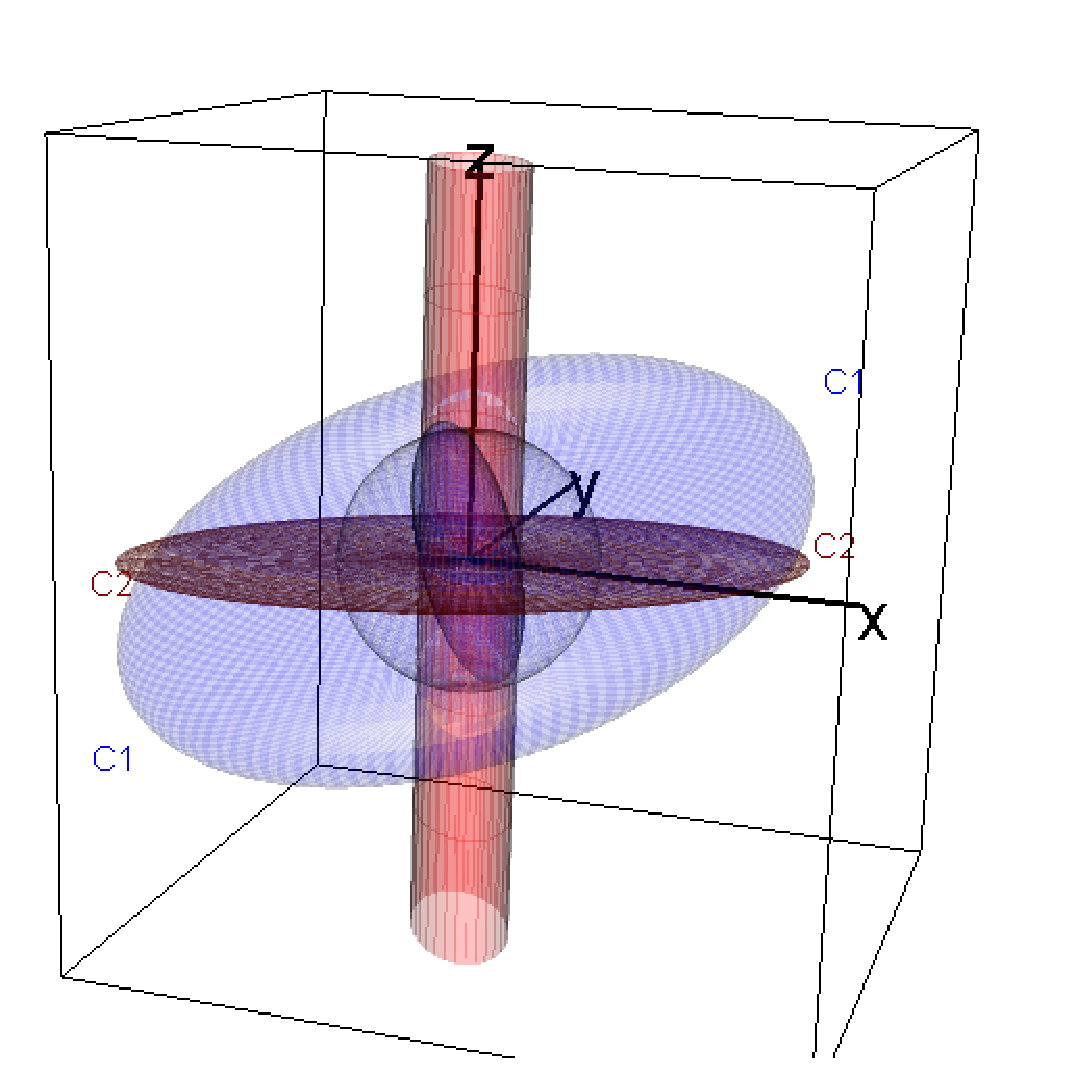
\includegraphics[width=1\linewidth]{fig/gell3d-1}
 \end{minipage}%
 \hfill
 \begin{minipage}[b]{.49\linewidth}
  \centering
  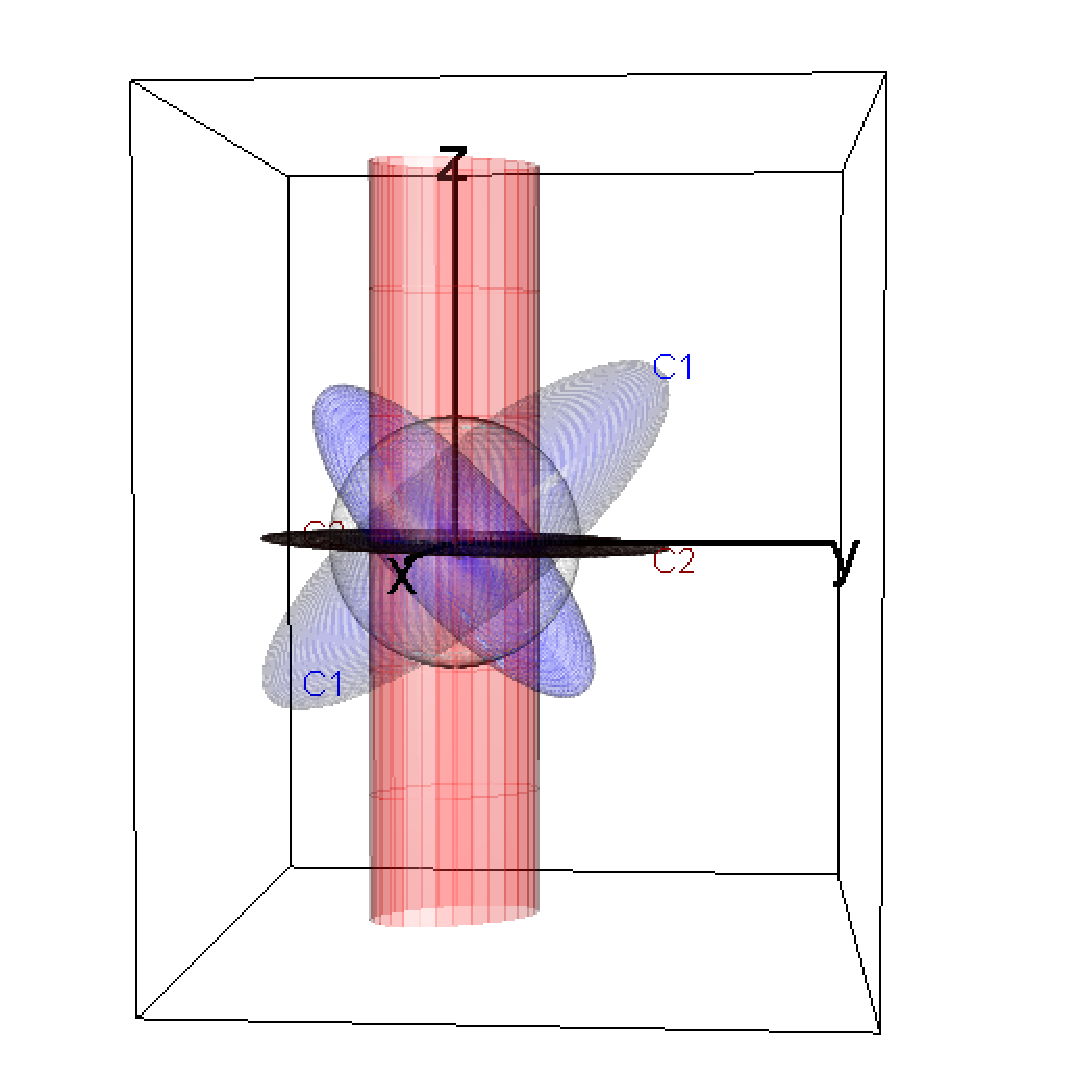
\includegraphics[width=1\linewidth]{fig/gell3d-4}
 \end{minipage}
\caption{Two views of an example of generalized ellipsoids.  $\mat{C}_1$  (blue) determines a proper, fat ellipsoid;
its inverse $\mat{C}_1^{-1}$ also generates a proper ellipsoid. $\mat{C}_2$  (red) determines an improper, flat ellipsoid,
whose inverse $\mat{C}_2^{-1}$ is an unbounded cylinder of elliptical cross section.  The scale of these images is defined
by a unit sphere (gray). The right panel shows a view illustrating the orthogonality of each $\mat{C}$ and its dual,  $\mat{C}^{-1}$.
}
\label{fig:gell3d}
\end{figure}

\figref{fig:gell3d} illustrates these ideas, using two generating matrices, $\mat{C}_1$ and $\mat{C}_2$ in this more
general representation,
\[
\mat{C}_1 = \left[
\begin{array}{ccc}
 6 & 2 & 1  \\
 2 & 3 & 2  \\
 1 & 2 & 2
\end{array}
\right]
\comma \quad\quad
\mat{C}_2 = \left[
\begin{array}{ccc}
 6 & 2 & 0  \\
 2 & 3 & 0  \\
 0 & 0 & 0
\end{array}
\right]
\]
where $\mat{C}_1$ generates a proper ellipsoid and $\mat{C}_2$ generates an improper, flat ellipsoid.
These varieties of ellipsoids are more easily seen in the 3D movies included in the online supplements.

%\TODO{Check this section: it is complete enough? Could it be trimmed?} 
% \subsection{Properties of geometric ellipsoids}\label{sec:properties}

\begin{itemize}
 \item Translation: An ellipsoid centered at $\vec{x}_0$ has the definition $\mathcal{E} := \{ \vec{x}: (\vec{x}-\vec{x}_0)\trans \mat{C} (\vec{x}-\vec{x}_0) =1
 \}$ or $\mathcal{E} := \vec{x}_0 \oplus\mat{A} \mathcal{S}$ in the notation of \secref{sec:statistical}.

 \item Orthogonality: If $\mat{C}$ is diagonal, then the origin-centered ellipsoid has its axes aligned with the coordinate axes and
has the equation
\begin{equation}\label{eq:ellisoid2}
 \vec{x}\trans \mat{C} \vec{x} = c_{11} x_1^2 + c_{22} x_2^2 + \cdots + c_{pp} x_p^2 =1 \comma
\end{equation}
where $1/\sqrt{c_{ii}} = c_{ii}^{-1/2}$ are the radii (semi-diameter lengths) along the coordinate axes.

 \item Area and volume: In two dimensions, the area of the axis-aligned ellipse is $\pi (c_{11} c_{22})^{-1/2}$.
 For $p=3$, the volume is $\frac{4}{3}\pi (c_{11} c_{22} c_{33})^{-1/2}$.
 In the general case, the hypervolume of the ellipsoid is proportional to $|\mat{C}|^{-1/2}=||\mat{A}||$
 and is given by $\pi^{p/2} \det{\mat{C}}^{-1/2} / \left[  \Gamma\left(\frac{p}{2}+1\right) \right]$
 \citep[\S 3.5]{Dempster:69}
% ($\mathcal{D}$ \S 3.5),
 where the first two factors are familiar as the normalizing constant of the multivariate normal 
 density function.

\begin{figure}[tb]
  \centering
  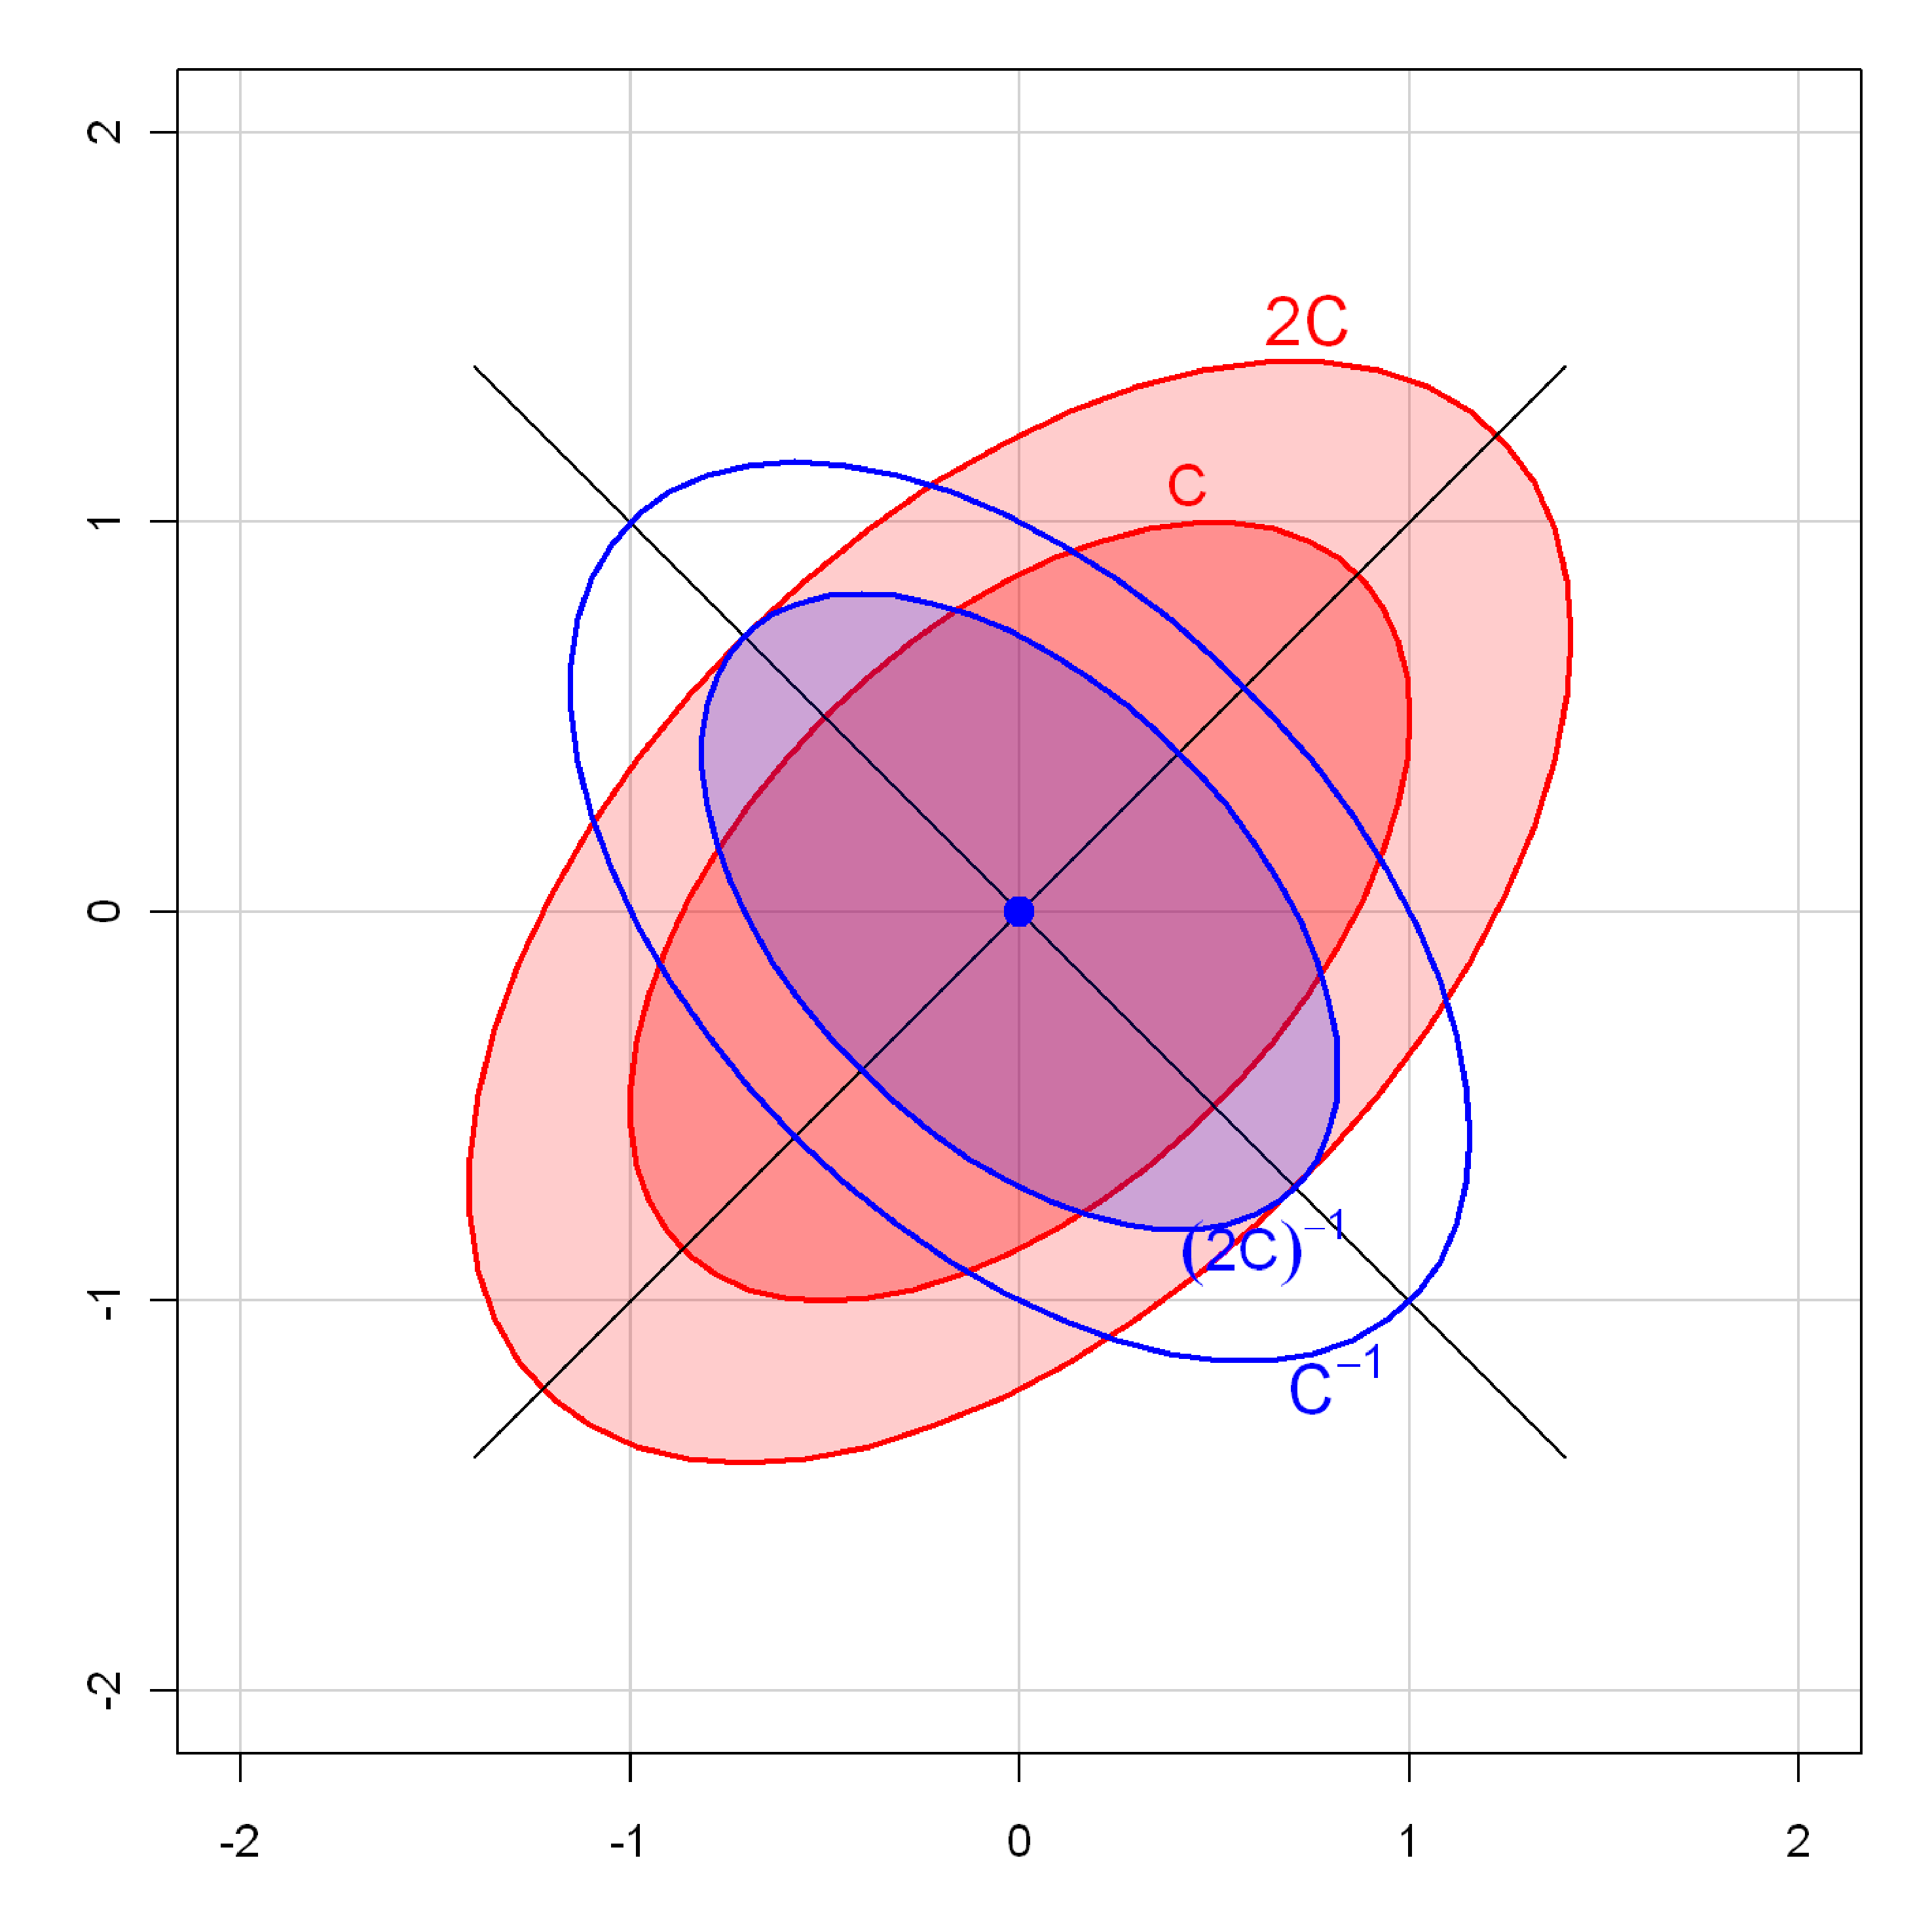
\includegraphics[width=.5\textwidth,clip]{fig/inverse}
  \caption{Some properties of geometric ellipsoids, shown in 2D. Principal axes of an ellipsoid are given by the eigenvectors of
  $\mat{C}$, with radii $1/\sqrt{\lambda_i}$.  For an ellipsoid defined by \eqref{eq:ellisoid1},
  the comparable ellipsoid for $2\mat{C}$ has radii multiplied by $1/\sqrt{2}$.
  The ellipsoid for $\mat{C}^{-1}$ has the same principal axes, but with radii $\sqrt{\lambda_i}$, making it
  small in the directions where $\mat{C}$ is large and vice-versa.
  } \label{fig:inverse}
\end{figure}

 \item Principal axes: In general, the eigenvectors, $\vec{v_i}, i=1,\dots,p$,
of $\mat{C}$ define the principal axes of the ellipsoid and
the inverse of the square roots of the ordered
eigenvalues, $\lambda_1 > \lambda_2 \dots, \lambda_p$, are the principal radii.
Eigenvectors belonging to eigenvalues that are 0 are directions in which the ellipsoid is unbounded.
With $\mathcal{E} = \mat{A} \mathcal{S}$, we consider the singular-value decomposition
$  \mat{A}= \mat{U} \mat{D} \mat{V} \trans$,
with $\mat{U}$ and  $\mat{V}$ orthogonal matrices and  $\mat{D}$  a diagonal non-negative matrix
with the same dimension as $\mat{A}$.
The column vectors of $\mat{U}$, called the left singular vectors,
correspond to the eigenvectors of $\mat{C}$ in the case of a proper ellipsoid.
The positive diagonal elements of $\mat{D}$, $d_1 > d_2 > ... > d_p>0$,
are the principal radii of the ellipsoid with $d_i = 1/\sqrt{\lambda_i}$.
In the singular case, the left singular vectors form a set of principal axes for the flattened ellipsoid.%
\footnote{Corresponding left singular vectors and eigenvectors are not necessarily equal, but sets that belong to the same eigenvalue/singular value span the same space.}

 \item Inverse: When $\mat{C}$ is positive definite, the eigenvectors of \mat{C} and $\mat{C}^{-1}$ are identical, while
the
 eigenvalues of $\mat{C}^{-1}$ are $1/\lambda_i$. It follows that the ellipsoid for
 $\mat{C}^{-1}$ has the same axes as that of $\mat{C}$, but with inversely proportional radii.
 In $\Real{2}$, the ellipsoid for $\mat{C}^{-1}$
 is, with rescaling, a \degree{90} rotation of the ellipsoid for $\mat{C}$,
 as illustrated in \figref{fig:inverse}.

 \item Generalized inverse: A definition for an inverse ellipsoid that is equivalent in the case of proper ellipsoids,
\begin{equation}\label{eq:ellipseginv}
\mathcal{E}^{-1} := \{ \vec{y} :   |\vec{x} \trans \vec{y}| \le 1 \comma \quad \forall \vec{x} \in \mathcal{E} \} \comma
\end{equation}
generalizes to all ellipsoids. The inverse of a singular ellipsoid is an improper ellipsoid and vice versa.

 \item Dimensionality: The ellipsoid is bounded if $\mat{C}$ is positive definite (all $\lambda_i > 0$).
 Each $\lambda_i = 0$ increases the dimension of the space along which the ellipsoid is unbounded by one.
For example, with $p=3$, $\lambda_3=0$ gives a
cylinder with an elliptical cross-section in 3-space, and  $\lambda_2 = \lambda_3=0$ gives an infinite slab with thickness $2 \sqrt{\lambda_1}$. With $\mathcal{E} = \mat{A} \mathcal{S}$, the dimension of the ellipsoid is equal to the number of positive singular values of $\mat{A}$.
 \item Projections: The projection of a $p$ dimensional ellipsoid into any subspace
is $\mat{P} \mathcal{E}$, where
$\mat{P}$ is an idempotent $p \times p$ (projection) matrix, i.e., $\mat{P} \mat{P}= \mat{P}^2 = \mat{P}$.
For example, in $\Real{2}$ and $\Real{3}$,
% $\Re^3$,
the matrices
\[
\mat{P}_2 =
\left[
\begin{array}{cc}
 1 & 1  \\
 0 & 0  \\
\end{array}
\right]
\comma \quad\quad
\mat{P}_3 =
\left[
\begin{array}{ccc}
 1 & 0 & 0 \\
 0 & 1 & 0 \\
 0 & 0 & 0 \\
\end{array}
\right]
\]
project, respectively, an ellipse onto the line $x_1 = x_2$, and an ellipsoid into the ($x_1, x_2$) plane.  If $\mat{P}$ is symmetric, then $\mat{P}$ is the matrix of an orthogonal projection, and it is easy to visualize  $\mat{P} \mathcal{E}$ as the shadow of  $\mathcal{E}$ cast perpendicularly onto  $\mathrm{span}(\mat{P})$. Generally,  $\mat{P} \mathcal{E}$ is the shadow of $\mathcal{E}$  onto  $\mathrm{span}(\mat{P})$ along the null space of $\mat{P}$.

 \item Linear transformations: A linear transformation of an ellipsoid is an ellipsoid, and the pre-image of an ellipsoid under a linear transformation is an ellipsoid.  
A non-singular linear transformation maps a proper ellipsoid into a proper ellipsoid in the form shown in \secref{sec:statistical}, \eqref{eq:Limage}. 

 \item Slopes and tangents: The slopes of the ellipsoidal surface in the directions of the coordinate
 axes are given by $\partial / \partial \vec{x} \: (\vec{x}\trans \mat{C} \vec{x}) = 2 \mat{C} \vec{x}$.
 From this, it follows that the tangent hyperplane to the unit ellipsoidal surface at the point
 $\vec{x}_\alpha$, where $\vec{x}_\alpha\trans \: \partial / \partial \vec{x} (\vec{x}\trans \mat{C} \vec{x}) = 0$,
 has the equation $\vec{x}_\alpha \trans \mat{C} \vec{x} = 1$.
\end{itemize}


% \subsection{Conjugate axes and inner-product spaces}\label{sec:conjugate}

For any non-singular $\mat{A}$ in \eqref{eq:ellAS} that generates an ellipsoid,  %% added non-singular / GM
the columns of
$\mat{A}=\left[
   \vec{a}_{1}, \vec{a}_{2}, \cdots, \vec{a}_{p}  \\
\right]
$
form a set of ``conjugate axes'' of the ellipse. (Two diameters are conjugate \emph{iff}
the tangent line at the endpoint of one diameter is parallel to the other diameter.)
Each vector
$\vec{a}_{i}$
lies on the ellipse, and the tangent hyperplane at that point is parallel to the span of all the other column vectors of
$\vec{A}$.
\begin{figure}[htb]
 \begin{minipage}[b]{.49\linewidth}
  \centering
  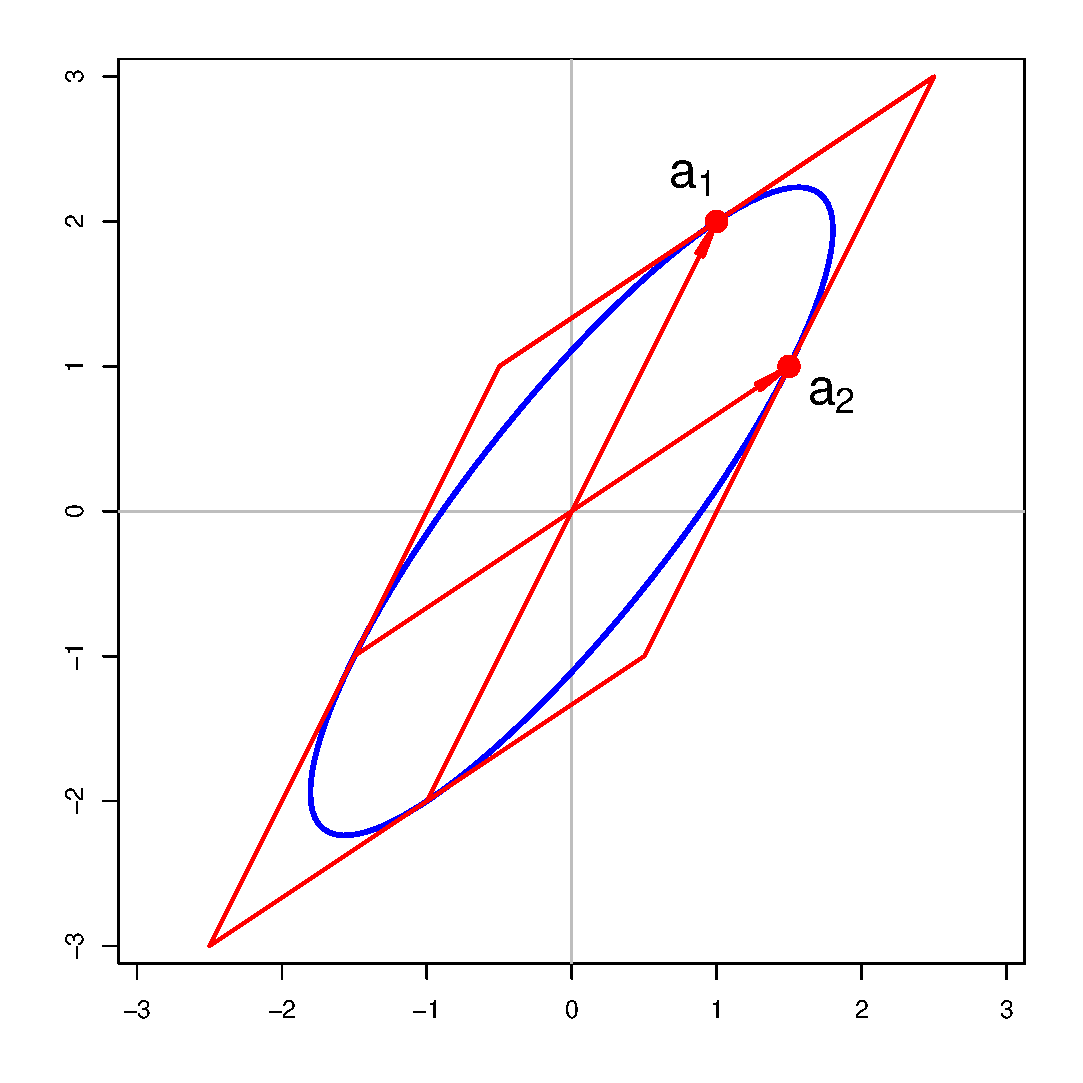
\includegraphics[width=1\linewidth]{fig/conjugate1}
 \end{minipage}%
 \hfill
 \begin{minipage}[b]{.49\linewidth}
  \centering
  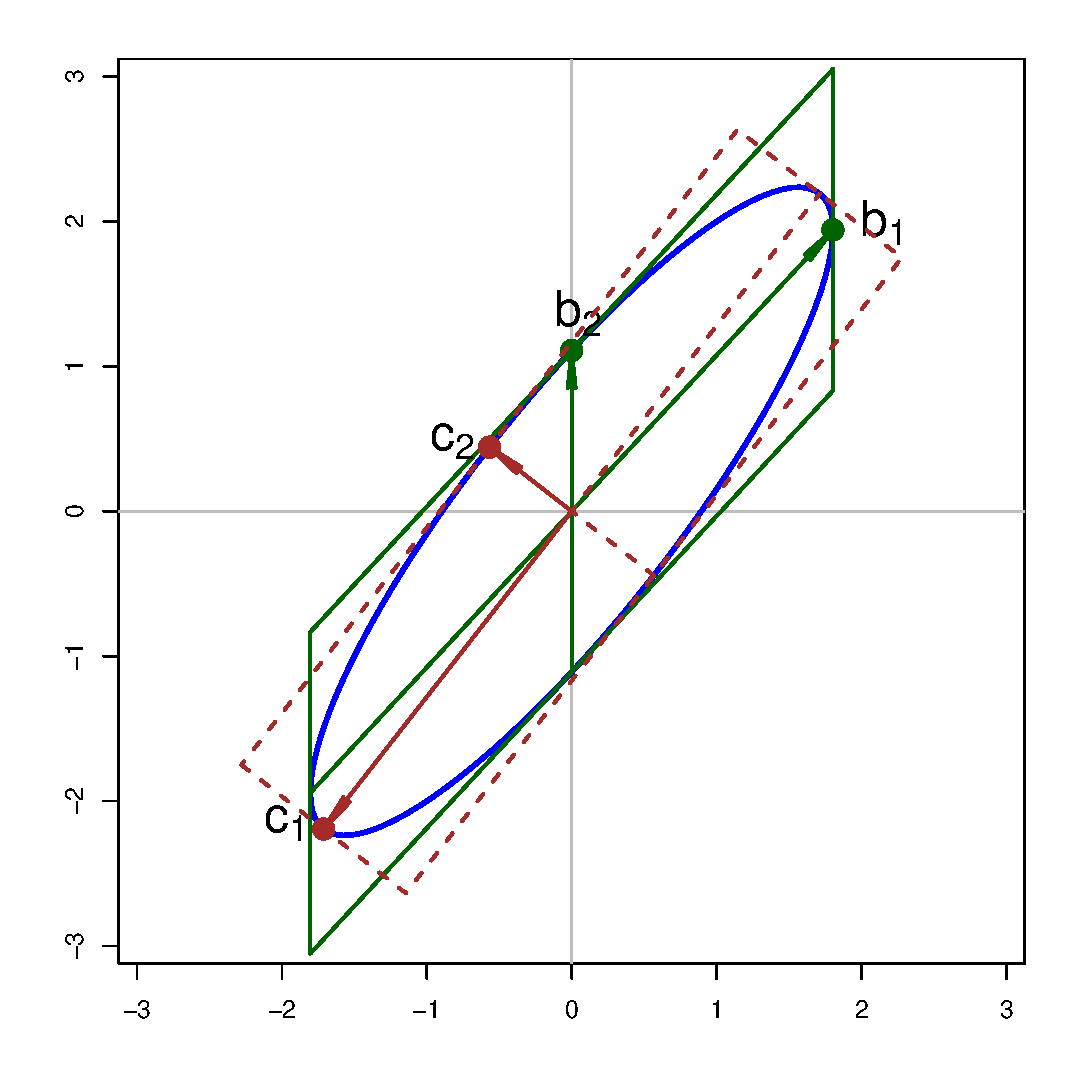
\includegraphics[width=1\linewidth]{fig/conjugate2}
 \end{minipage}
\caption{Conjugate axes of an ellipsoid with various factorizations of $\mat{W}$ and corresponding
basis vectors.
The conjugate vectors lie on the ellipsoid, and their tangents can be extended to form a parallelogram framing it.
Left: for an arbitrary factorization, given in \eqref{eq:fac1}.
Right: for the Choleski factorization (solid, green, $b_1, b_2$) and the principal component factorization (dashed, brown, $c_1, c_2$).
}
\label{fig:conjugate}
\end{figure}
For
$p=2$
this result is illustrated in \figref{fig:conjugate} (left)
in which

\begin{equation}\label{eq:fac1}
\mat{A}=\left[ \begin{matrix}
   \vec{a}_{1} & \mat{a}_{2}  \\
\end{matrix} \right]=\left[
\begin{matrix}
   1 & 1.5  \\
   2 & 1  \\
\end{matrix} \right]
\mbox{   }\Rightarrow\mbox{   }
\mat{W}=\mat{A A\trans}=
\left[ \begin{matrix}
   3.25 & 3.5  \\
   3.5 & 5  \\
\end{matrix} \right]
\period
\end{equation}

Consider the inner-product space with inner product matrix 	
$\mat{W}^{-1}=\left[ \begin{matrix}	
1.25 & -0.875 \\	
-0.875 & 0.8125 \\	
\end{matrix} \right]
$ and inner product	
\begin{equation*}
\left\langle \vec{x},\vec{y} \right\rangle =\vec{{x}'W}^{-1}\vec{y} \period
\end{equation*} 	
Because	
$\mat{A}\trans \mat{W}^{-1}\mat{A}
=\mat{A}\trans\left( \mat{A}\mat{A}\trans \right)^{-1}\mat{A}
=\mat{A}\trans(\mat{A}\trans)^{-1}\mat{A}^{-1}\mat{A}
=\mat{I}
$,
we see that
$\vec{a}_{1}$
and	
$\vec{a}_{2}$	
are orthogonal unit vectors (in fact, an orthonormal basis) in this inner product:	

\begin{eqnarray*}
\left\langle \vec{a}_{i},\vec{a}_{i} \right\rangle & = & \vec{{a}\trans}_{i}\mat{W}^{-1}\vec{a}_{i}=1	 \\
%	
\left\langle \vec{a}_{1},\vec{a}_{2} \right\rangle & = &\vec{{a}'}_{1}\mat{W}^{-1}\vec{a}_{2}=0 \period
\end{eqnarray*}


Now, if $\mat{W}=\mat{B{B}\trans}$ is any other factorization of
$\mat{W}$,
then the columns of
$\mat{B}$
have the same properties as the columns of
$\mat{A}$.
Particular factorizations yield interesting and statistically useful sets of conjugate axes.
The illustration in \figref{fig:conjugate} (right) shows two such cases with special properties:
In the Choleski factorization (shown solid in green), where
$\mat{B}$ is lower triangular, the last conjugate axis, $\vec{b}_2$, is aligned with the coordinate
axis $\vec{x}_2$.  Each previous axis ($\vec{b}_1$, here) is the orthogonal complement to
all later axes in the  inner-product space of
$\mat{W}^{-1}$.  
The Choleski factorization is unique in this respect, subject to a
permutation of the rows and columns of \mat{W}. 
The subspace $\{ c_1 \vec{b}_1 + ... + c_{p-1} \vec{b}_{p-1}  , c_i \in \mathbb{R}\}$, is the plane of the regression of the last variable on the others, a fact that generalizes naturally to ellipsoids that are not necessarily centerered at the origin.  %% added fact /GM  

In the principal-component (PC) factorization (shown dashed in brown) $\mat{W}=\mat{C} \mat{C}\trans$, where
$\mat{C}=\mat{\Gamma \Lambda }^{1/2}$
and hence
$\mat{W}=\mat{\Gamma \Lambda {\Gamma }'}$
is the spectral decomposition of
$\mat{W}$. Here, the ellipse axes are orthogonal in the space of the ellipse
(so the bounding tangent parallelogram is a rectangle) \emph{as well as} in the inner-product space of
$\mat{W}^{-1}$. The PC factorization is unique in this respect (up to reflections of the axis vectors).

As illustrated in \figref{fig:conjugate}, each pair of conjugate axes has a corresponding bounding tangent
parallelogram. It can be shown that all such parallelograms have the same area
and equal sums of squares of the lengths of their diameters.

% \subsection{Ellipsoids in a generalized metric space}

%\todo{Georges?}
%\TODO{Smooth out and simplify this description. Add to the plot: unit vectors in data space, and their transformations in canonical space.
%Here it would be useful to describe the geometric relations that pertain to \mat{H}
%(positive semi-definite)
%in the metric of \mat{E} (positive definite).
%I see two sub-figures:
%(a) ellipses for \mat{H} and \mat{E}, showing the conjugate axes and
%bounding parallelogram for \mat{E}, perhaps using the principal component factorization.
%(b) the transformation of (a) using $\mat{H}\mat{E}^{-1}$ or
%$\mat{E}^{-1/2} \, \mat{H} \, \mat{E}^{-1/2}$.
%}

In the discussion above, we considered the positive semi-definite matrix \mat{W} and
corresponding ellipsoid to be
referred to a Euclidean space, perhaps with different basis vectors.
We showed that various measures of the ``size'' of the ellipsoid could be defined
in terms of functions of the eigenvalues $\lambda_i$ of \mat{W}.

We now consider the generalized
case of an analogous $p \times p$ positive semi-definite symmetric matrix \mat{H}, but where measures of
length, distance, and angles are referred to a metric defined by a positive-definite symmetric
matrix \mat{E}. As is well known, the generalized eigenvalue problem is to find the scalars
$\lambda_i$ and vectors $\vec{v}_i, i=1, 2, \dots p$,
such that $\mat{H} \vec{v} = \lambda \mat{E} \vec{v}$, that is, the roots of
$\det{\mat{H} - \lambda \mat{E}}=0$.

%\TODO{More explanation here ...}
\begin{figure}[htb]
% two figs side-by-side
  \begin{minipage}[c]{.495\textwidth}
   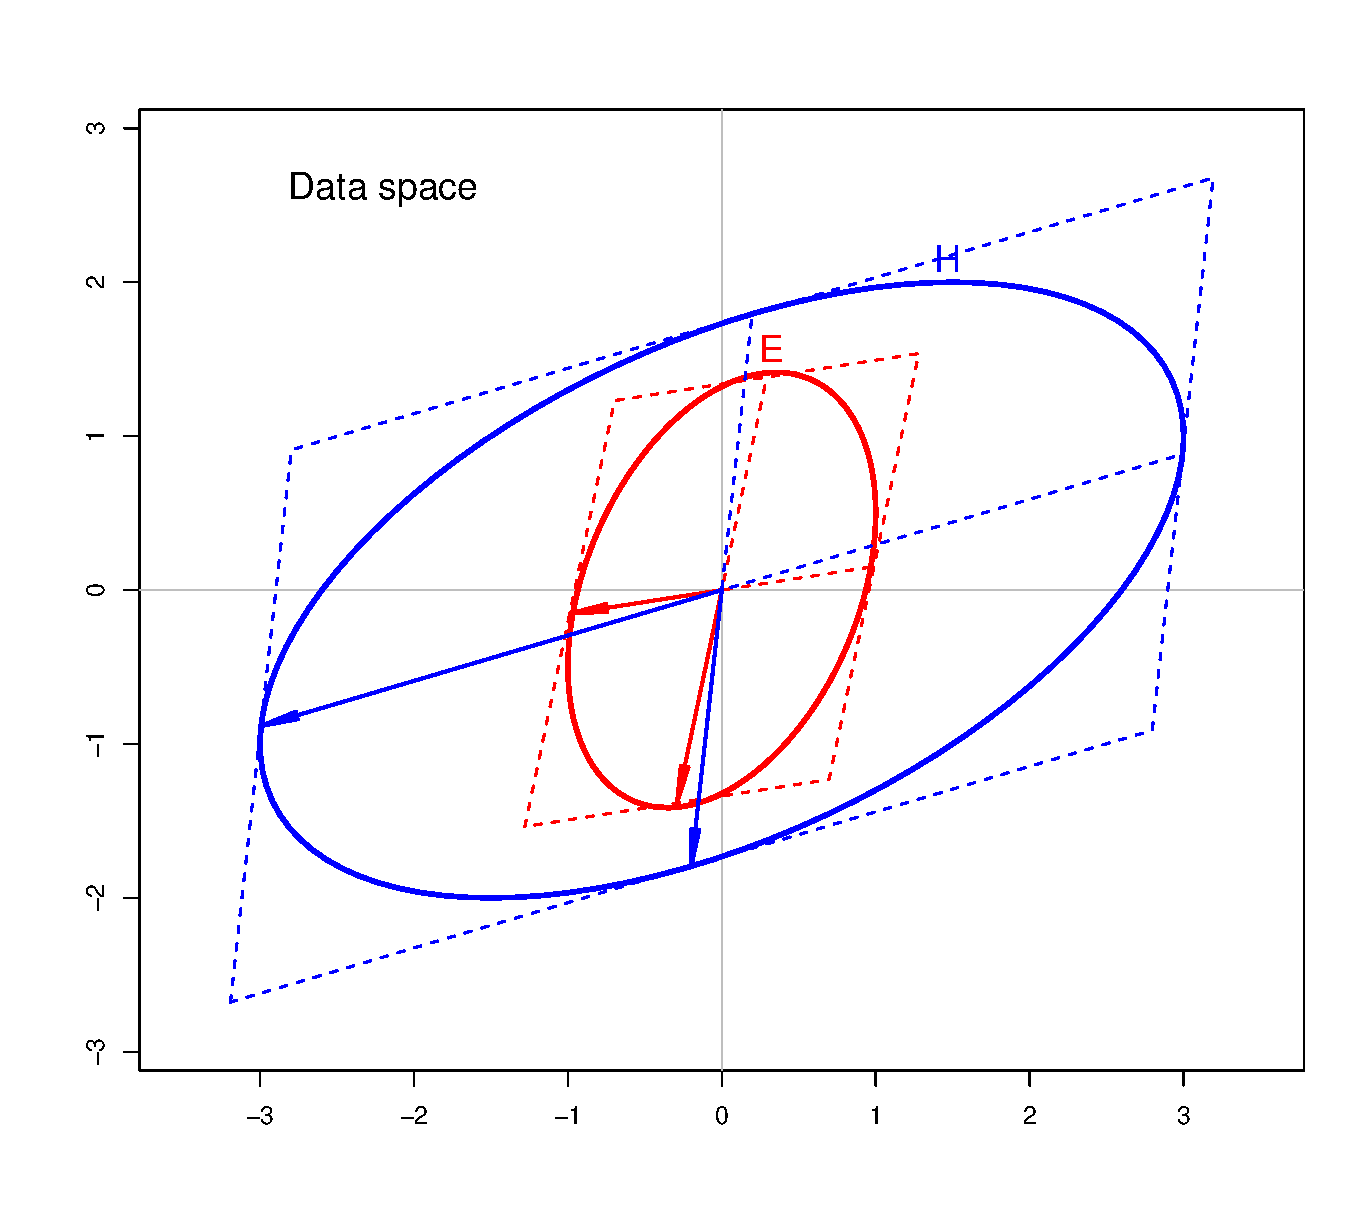
\includegraphics[width=1\linewidth,clip]{fig/ellipse-geneig1}
   \end{minipage}%
  \hfill
  \begin{minipage}[c]{.495\textwidth}
   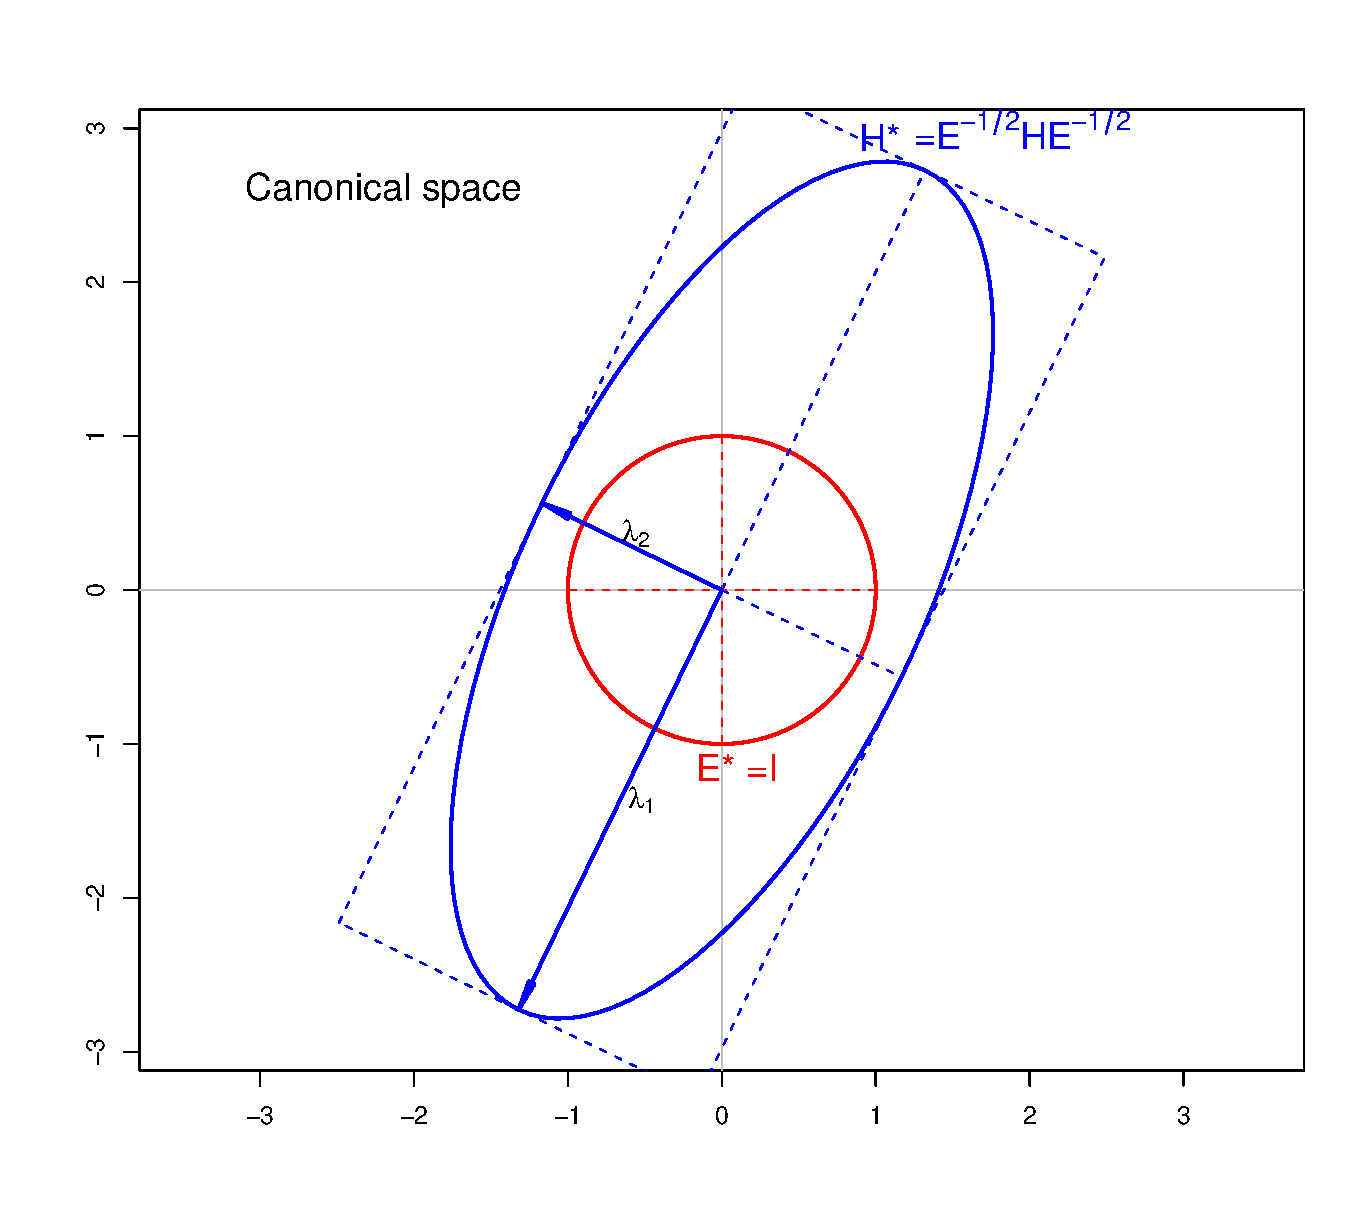
\includegraphics[width=1\linewidth,clip]{fig/ellipse-geneig2}
  \end{minipage}
  \caption{Left: Ellipses for \mat{H} and \mat{E} in Euclidean ``data space,''
   Right: Ellipses for $\mat{H}^\star$ and $\mat{E}^\star$ in the transformed ``canonical space,''
   with the eigenvectors of \mat{H} relative to \mat{E} shown as blue arrows, whose radii
   are the corresponding eigenvalues, $\lambda_1, \lambda_2$. }%
  \label{fig:ellipse-geneig}
\end{figure}
For such \mat{H} and \mat{E}, we can always find a factor \mat{A} of \mat{E}, so that
$\mat{E} = \mat{A} \mat{A}\trans$, whose colums will be conjugate directions for \mat{E}
and whose rows will also be conjugate directions for \mat{H}, in that $\mat{H} = \mat{A}\trans \mat{D} \mat{A}$,
where $\mat{D}$ is diagonal.  Geometrically, this means that there exists a unique pair of
bounding parallelograms for the \mat{H} and \mat{E} ellipsoids whose
corresponding sides are parallel. A linear transformation of \mat{E} and \mat{H}
that transforms the parallelogram
for \mat{E} to a square (or cuboid), and hence \mat{E} to a sphere (or spheroid), generates an
equivalent view in what we describe below as canonical space.


In statistical applications (e.g., MANOVA, canonical correlation), the generalized
eigenvalue problem is transformed to an ordinary eigenvalue problem by considering
the following equivalent forms with the same $\lambda_i$, $\vec{v}_i$,
\begin{eqnarray*}
(\mat{H} - \lambda \mat{E}) \vec{v} & = & \vec{0} \\
\Rightarrow (\mat{H} \, \inv{\mat{E}} - \lambda \mat{I}) \vec{v} & = & \vec{0} \\
\Rightarrow (\invhalf{\mat{E}} \, \mat{H} \, \invhalf{\mat{E}} - \lambda \mat{I}) \vec{v} & = & \vec{0} \comma
\end{eqnarray*}
where the last form gives a symmetric matrix, $\mat{H}^\star = \invhalf{E} \, \mat{H} \, \invhalf{E}$.
Using the square root of \mat{E} defined by the
principal-component factorization $\half{E} = \mat{\Gamma} \half{\mat{\Lambda}}$ produces
the ellipsoid of $\mat{H}^\star$
orthogonal axes corresponding to the $\vec{v}_i$, whose squared radii are the corresponding %% squared / GM
eigenvalues $\lambda_i$.  This can be seen geometrically as a rotation of ``data space''
to an orientation defined by the principal axes of \mat{E}, followed by a re-scaling, so
that the \mat{E} ellipsoid becomes the unit spheroid.  In this transformed space
(``canonical space''), functions of the
the squared radii $\lambda_i$ of the axes of $\mat{H}^\star$ give direct measures of %% squared / GM
the ``size'' of \mat{H} relative to \mat{E}. The orientation of the eigenvectors
$\vec{v}_i$ can be related to the (orthogonal) linear combinations of the
data variables that are successively largest in the metric of \mat{E}.


To illustrate, \figref{fig:ellipse-geneig} (left) shows
the ellipses generated by
\begin{equation*}
 \mat{H} = \left[ \begin{array}{cc}
                   9 & 3 \\
                   3 & 4
                  \end{array}\right]
 \quad \mbox{ and } \quad
 \mat{E} = \left[ \begin{array}{cc}
                   1 & 0.5 \\
                   0.5 & 2
                  \end{array}\right]
\end{equation*}
together with their conjugate axes. For \mat{E}, the conjugate axes are defined by the columns of the right factor,
$\mat{A}\trans$,
in $\mat{E} = \mat{A} \mat{A}\trans$; for \mat{H}, the conjugate axes are defined by the columns of $\mat{A}$.
The transformation to $\mat{H}^\star = \invhalf{E} \, \mat{H} \, \invhalf{E}$ is shown in the right panel
of \figref{fig:ellipse-geneig}. In this ``canonical space,'' angles and lengths have the orginary interpretation
of Euclidean space, so the size of $\mat{H}^\star$ can be interpreted directly in terms of functions of
the radii $\sqrt{\lambda_1}$ and $\sqrt{\lambda_2}$.



%\bibliography{timeref,graphics,Rpackages,statistics}
\bibliography{supp}        % processed by bibtool -- quiet=on -r ~/texmf/bibtex/bib/aux2bib.rsc -x supp.aux -o supp.bib

\end{document}

